% Generated by tools/md_to_tex.py from ../rrrrrreporrrrrrt.md.
% Edit the markdown source or the converter, then run `make content`.

\section{0. Introduzione al Progetto}
\label{sec:0-introduzione-al-progetto}

Questo progetto si svolge nel più ampio contesto del corso di Statistica Applicata nel CdL in Ingegneria Informatica all'Università di Salerno.

Ci è stato fornito un dataset rappresentativo di un campione dei quali elementi consideriamo 8 caratteristiche, una di queste è espressa come dipendente dalle altre.

L'obiettivo di questa attività è quello di svolgere un'analisi statistica descrittiva sui dati forniti, per poi procedere con una fase di regressione lineare multipla, al fine di identificare un modello che possa spiegare al meglio la variabilità della variabile dipendente in funzione delle altre caratteristiche.

Al termine dell'attività potremo fornire a un ipotetico operatore le conoscenze necessarie per ottimizzare la procedura di acquisizioni di immagini da UAV.

\section{1. Analisi Statistica Descrittiva}
\label{sec:1-analisi-statistica-descrittiva}

Nella sezione di Statistica Descrittiva andremo a utilizzare una serie di strumenti per valutare la natura dei dati forniti. Questi strumenti permettono di ottenere insight sui dati presentati, che verranno usati per guidare le fasi successive del progetto.

Il campione in analisi è costituito da 100 (\texttt{\detokenize{n = nrow(ds)}}) elementi di cui sono definite 8 caratteristiche di natura quantitativa continua.

Per avere un'idea limitata ma immediata della natura dei dati, abbiamo visualizzato i valori iniziali e finali del campione, ordinati secondo la variabile dipendente \texttt{\detokenize{y_IQ}}.

\begin{lstlisting}[style=rconsole,caption={head(twist\_sorted)}]
      y_IQ      x1_ISO       x2_T       x3_MP
  85.76275  1.71051927  1.2694487 -1.60960262
  89.37733  0.47531620  1.6607291  0.01548673
  91.74121  1.61621307  1.6178761  0.94264143
  94.66445  1.43905003  1.4720261 -1.06032801
 101.76777  0.01069104  1.5602105 -1.71690096
 104.91759  1.40622836  0.6077778  0.20020511
     x4_CF        x5_F     x6_GSI       x7_UA
-0.5973638  1.21935086  0.9950725  -1.2313230
-0.3395450  2.11793190  1.5027906  -1.6492509
-1.5664503 -1.95141132  0.7572437  -0.2628265
 0.7965453  0.03008541 -0.6582414  -0.7980054
 1.2178391  0.46207915  0.7841440  -1.1420552
-0.1788123  1.62989182  0.4556526   1.4947013
\end{lstlisting}

\begin{lstlisting}[style=rconsole,caption={tail(twist\_sorted)}]
      y_IQ     x1_ISO        x2_T      x3_MP
  166.9723  0.1009377 -0.09395068  1.2803254
  168.0356 -0.2722747  0.58255508 -0.3704142
  172.9470 -1.7186148 -1.02359897  1.4190216
  174.0162 -1.0760703 -1.57173461  1.4307073
  178.1100 -1.6223626 -1.28167295  0.3701268
  181.1781 -1.6345881 -1.50141175  0.2449209
     x4_CF       x5_F     x6_GSI       x7_UA
-0.1025210 -0.8338555 -0.7336588 -0.19635859
-0.4599907 -0.3538943 -1.6650442  0.46473235
-1.5514532 -1.4660646 -1.4374694  0.79578587
 0.3972056 -0.9538855 -0.6366092 -0.08404836
 0.7842828 -0.8365009 -0.2303526  0.29413924
 1.3692702 -0.7514527 -1.0163686 -0.88874785
\end{lstlisting}

\subsection{1.1. Summary \& Whiskers}
\label{sec:11-summary-whiskers}

Prima di tutto valutiamo gli indici di tendenza centrale (media e mediana) e di dispersione (deviazione standard) per tutte le caratteristiche del dataset.

\begin{lstlisting}[style=rconsole,caption={summary}]
      y_IQ                x1_ISO                x2_T
 Min.   :  85.76      Min.   :-1.71861     Min.   :-1.57489
 1st Qu.: 117.65      1st Qu.:-0.60159     1st Qu.:-0.91172
 Median : 135.13      Median : 0.08236     Median :-0.10059
 Mean   : 134.27      Mean   : 0.06321     Mean   :-0.04587
 3rd Qu.: 148.53      3rd Qu.: 0.90001     3rd Qu.: 0.69212
 Max.   : 181.18      Max.   : 1.72094     Max.   : 1.66073
     x3_MP                x4_CF                 x5_F
 Min.   :-1.7278494   Min.   :-1.65848     Min.   :-2.1460
 1st Qu.:-0.7305715   1st Qu.:-0.71533     1st Qu.:-0.7686
 Median : 0.0963404   Median :-0.08772     Median :-0.1531
 Mean   :-0.0002303   Mean   :-0.02413     Mean   : 0.0000
 3rd Qu.: 0.7124093   3rd Qu.: 0.81905     3rd Qu.: 0.6915
 Max.   : 1.7311851   Max.   : 1.72493     Max.   : 2.4726
     x6_GSI             x7_UA
 Min.   :-1.71454     Min.   :-1.6839
 1st Qu.:-0.90640     1st Qu.:-1.0527
 Median :-0.30275     Median :-0.1906
 Mean   :-0.09797     Mean   :-0.1496
 3rd Qu.: 0.78453     3rd Qu.: 0.6444
 Max.   : 1.70911     Max.   : 1.6263
\end{lstlisting}

\begin{lstlisting}[style=rconsole,caption={deviazione standard e varianza}]
                StD        Var
y_IQ        20.3977   416.0670
x1_ISO       1.0159     1.0321
x2_T         0.9618     0.9251
x3_MP        0.9746     0.9498
x4_CF        0.9741     0.9490
x5_F         1.0000     1.0000
x6_GSI       0.9879     0.9759
x7_UA        0.9997     0.9995
\end{lstlisting}

Notiamo che le variabili indipendenti presentano una deviazione standard prossima ad 1, ed una media prossima a 0, il che suggerisce che si possa trattare di dati standardizzati. La variabile dipendente invece è definita nel range [85.76, 181.18], per cui ne possiamo valutare il coefficiente di variazione (\texttt{\detokenize{sd(y_IQ) / mean(y_IQ)}}), che si attesta attorno al 15\%.

Queste informazioni possono essere analizzate in maniera efficace mediante l'utilizzo dei boxplot. Si sceglie di visualizzarne i notch e si tiene conto del fatto che il numero di osservazioni è uguale per tutte le variabili, per cui l'uso di \texttt{\detokenize{varwidth}} è indifferente.

\begin{figure}[H]
\centering
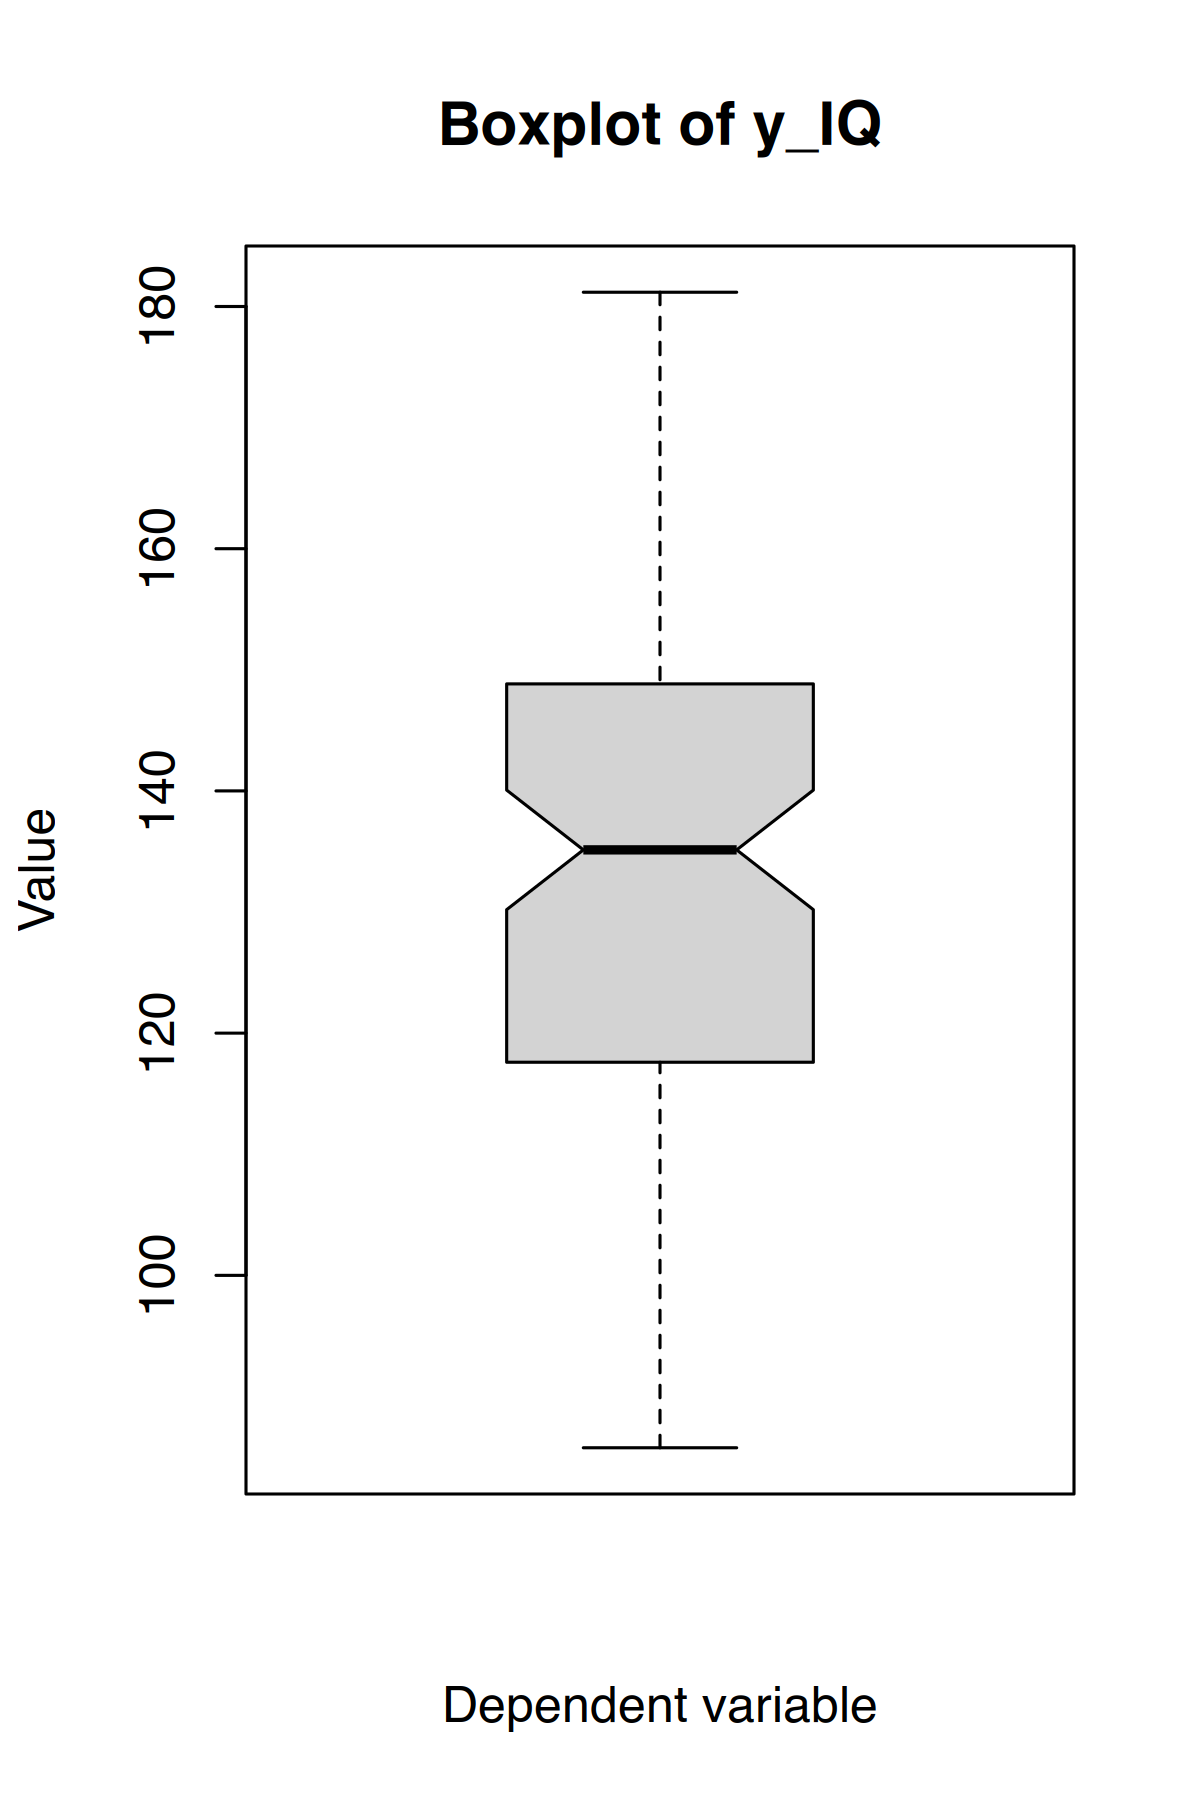
\includegraphics[width=0.30
\linewidth]{figures/plottwists/boxplot_y.png}
\hfill
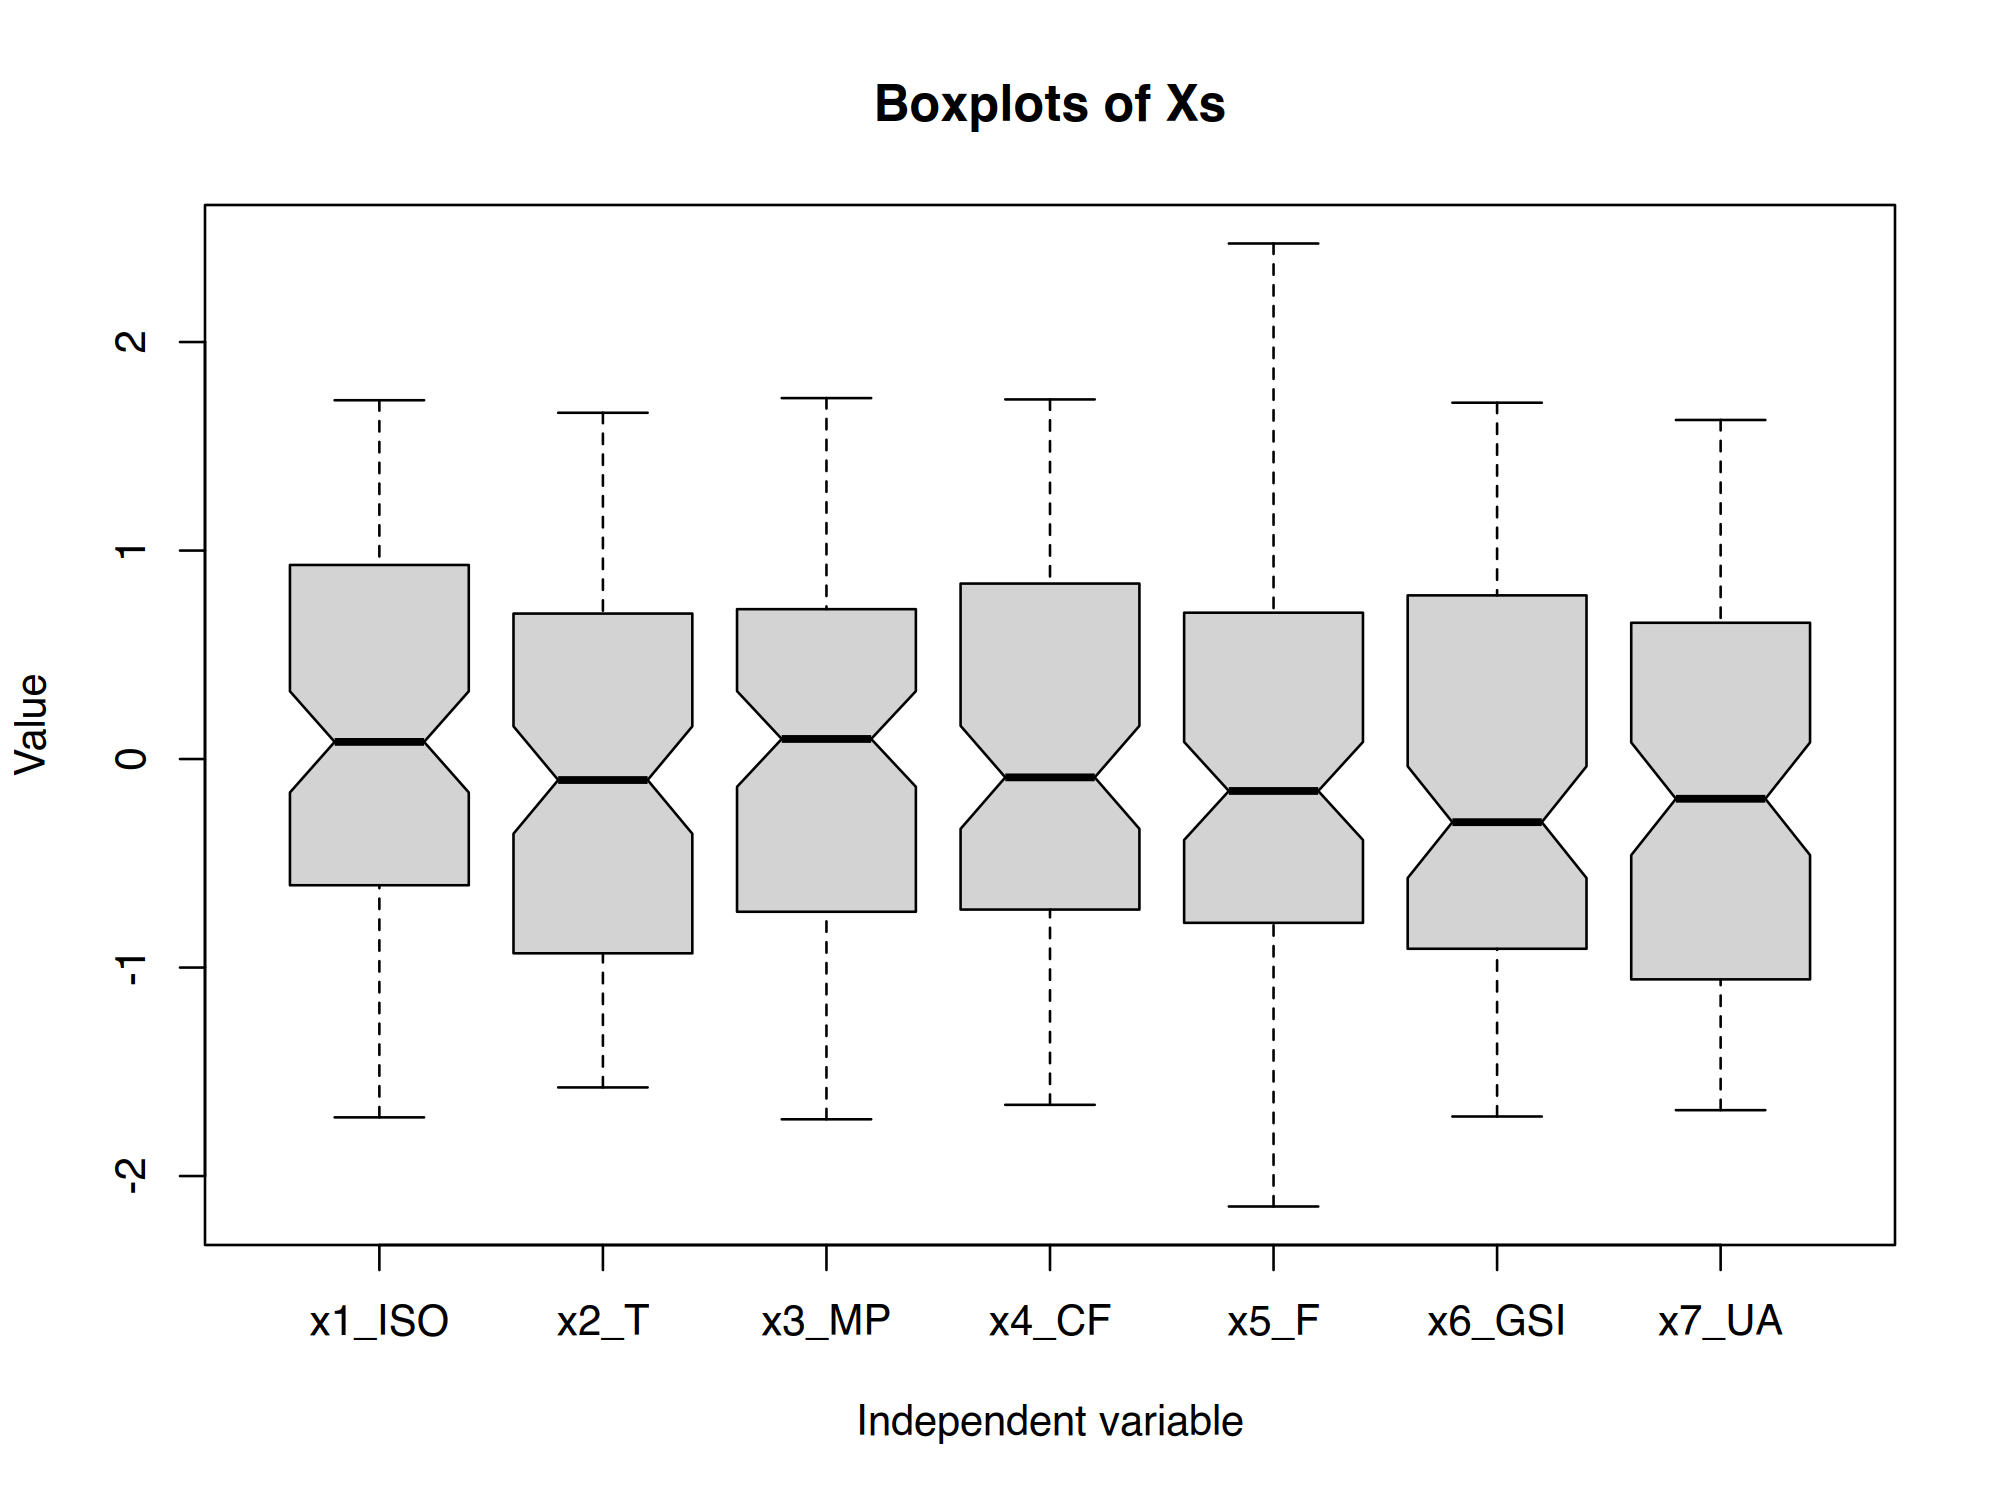
\includegraphics[width=0.60\linewidth]{figures/plottwists/boxplots_xs.png}
\caption{boxplot y / boxplots xs}
\end{figure}

Si nota:

\begin{itemize}
\item l'assenza di outliers prima di $\text{Q1} - 1.5\cdot\text{IQR}$ e oltre $\text{Q3} + 1.5\cdot\text{IQR}$ per tutte le variabili considerate, con influenza sulla lunghezza dei baffi
\begin{itemize}
\item la variabile \texttt{\detokenize{x5_F}} ha un'escursione campionaria particolarmente superiore alle altre, nonostante un IQR (range Q1-Q3) tra i più piccoli
\end{itemize}
\item le notch di tutte le variabili indipendenti tendono a sovrapporsi, che rende possibile eventuali uguaglianze tra mediane
\end{itemize}

\subsection{1.2. Istogrammi e Q-Q plot}
\label{sec:12-istogrammi-e-q-q-plot}

Per una sintesi visiva della distribuzione di frequenza dei valori delle caratteristiche prese in considerazione si può fare uso di istogrammi. Ricordando che l'informazione è di tipo quantitativo continuo, c'è la necessità di definire il numero di classi (k) in cui suddividere l'intervallo di osservazione. Di norma si procede con la relazione empirica di Sturges ($k = \lceil1 + 3.3 \cdot \log_{10}{n}\rceil$), o seguendo la norma UNI 4724-66 (secondo cui per una numerosità campionaria fino a 100 elementi si usano massimo 8 classi, 10 fino a 250), ma il comando \texttt{\detokenize{hist()}} determina i confini in maniera che risultino facili da leggere.

\begin{figure}[H]
\centering
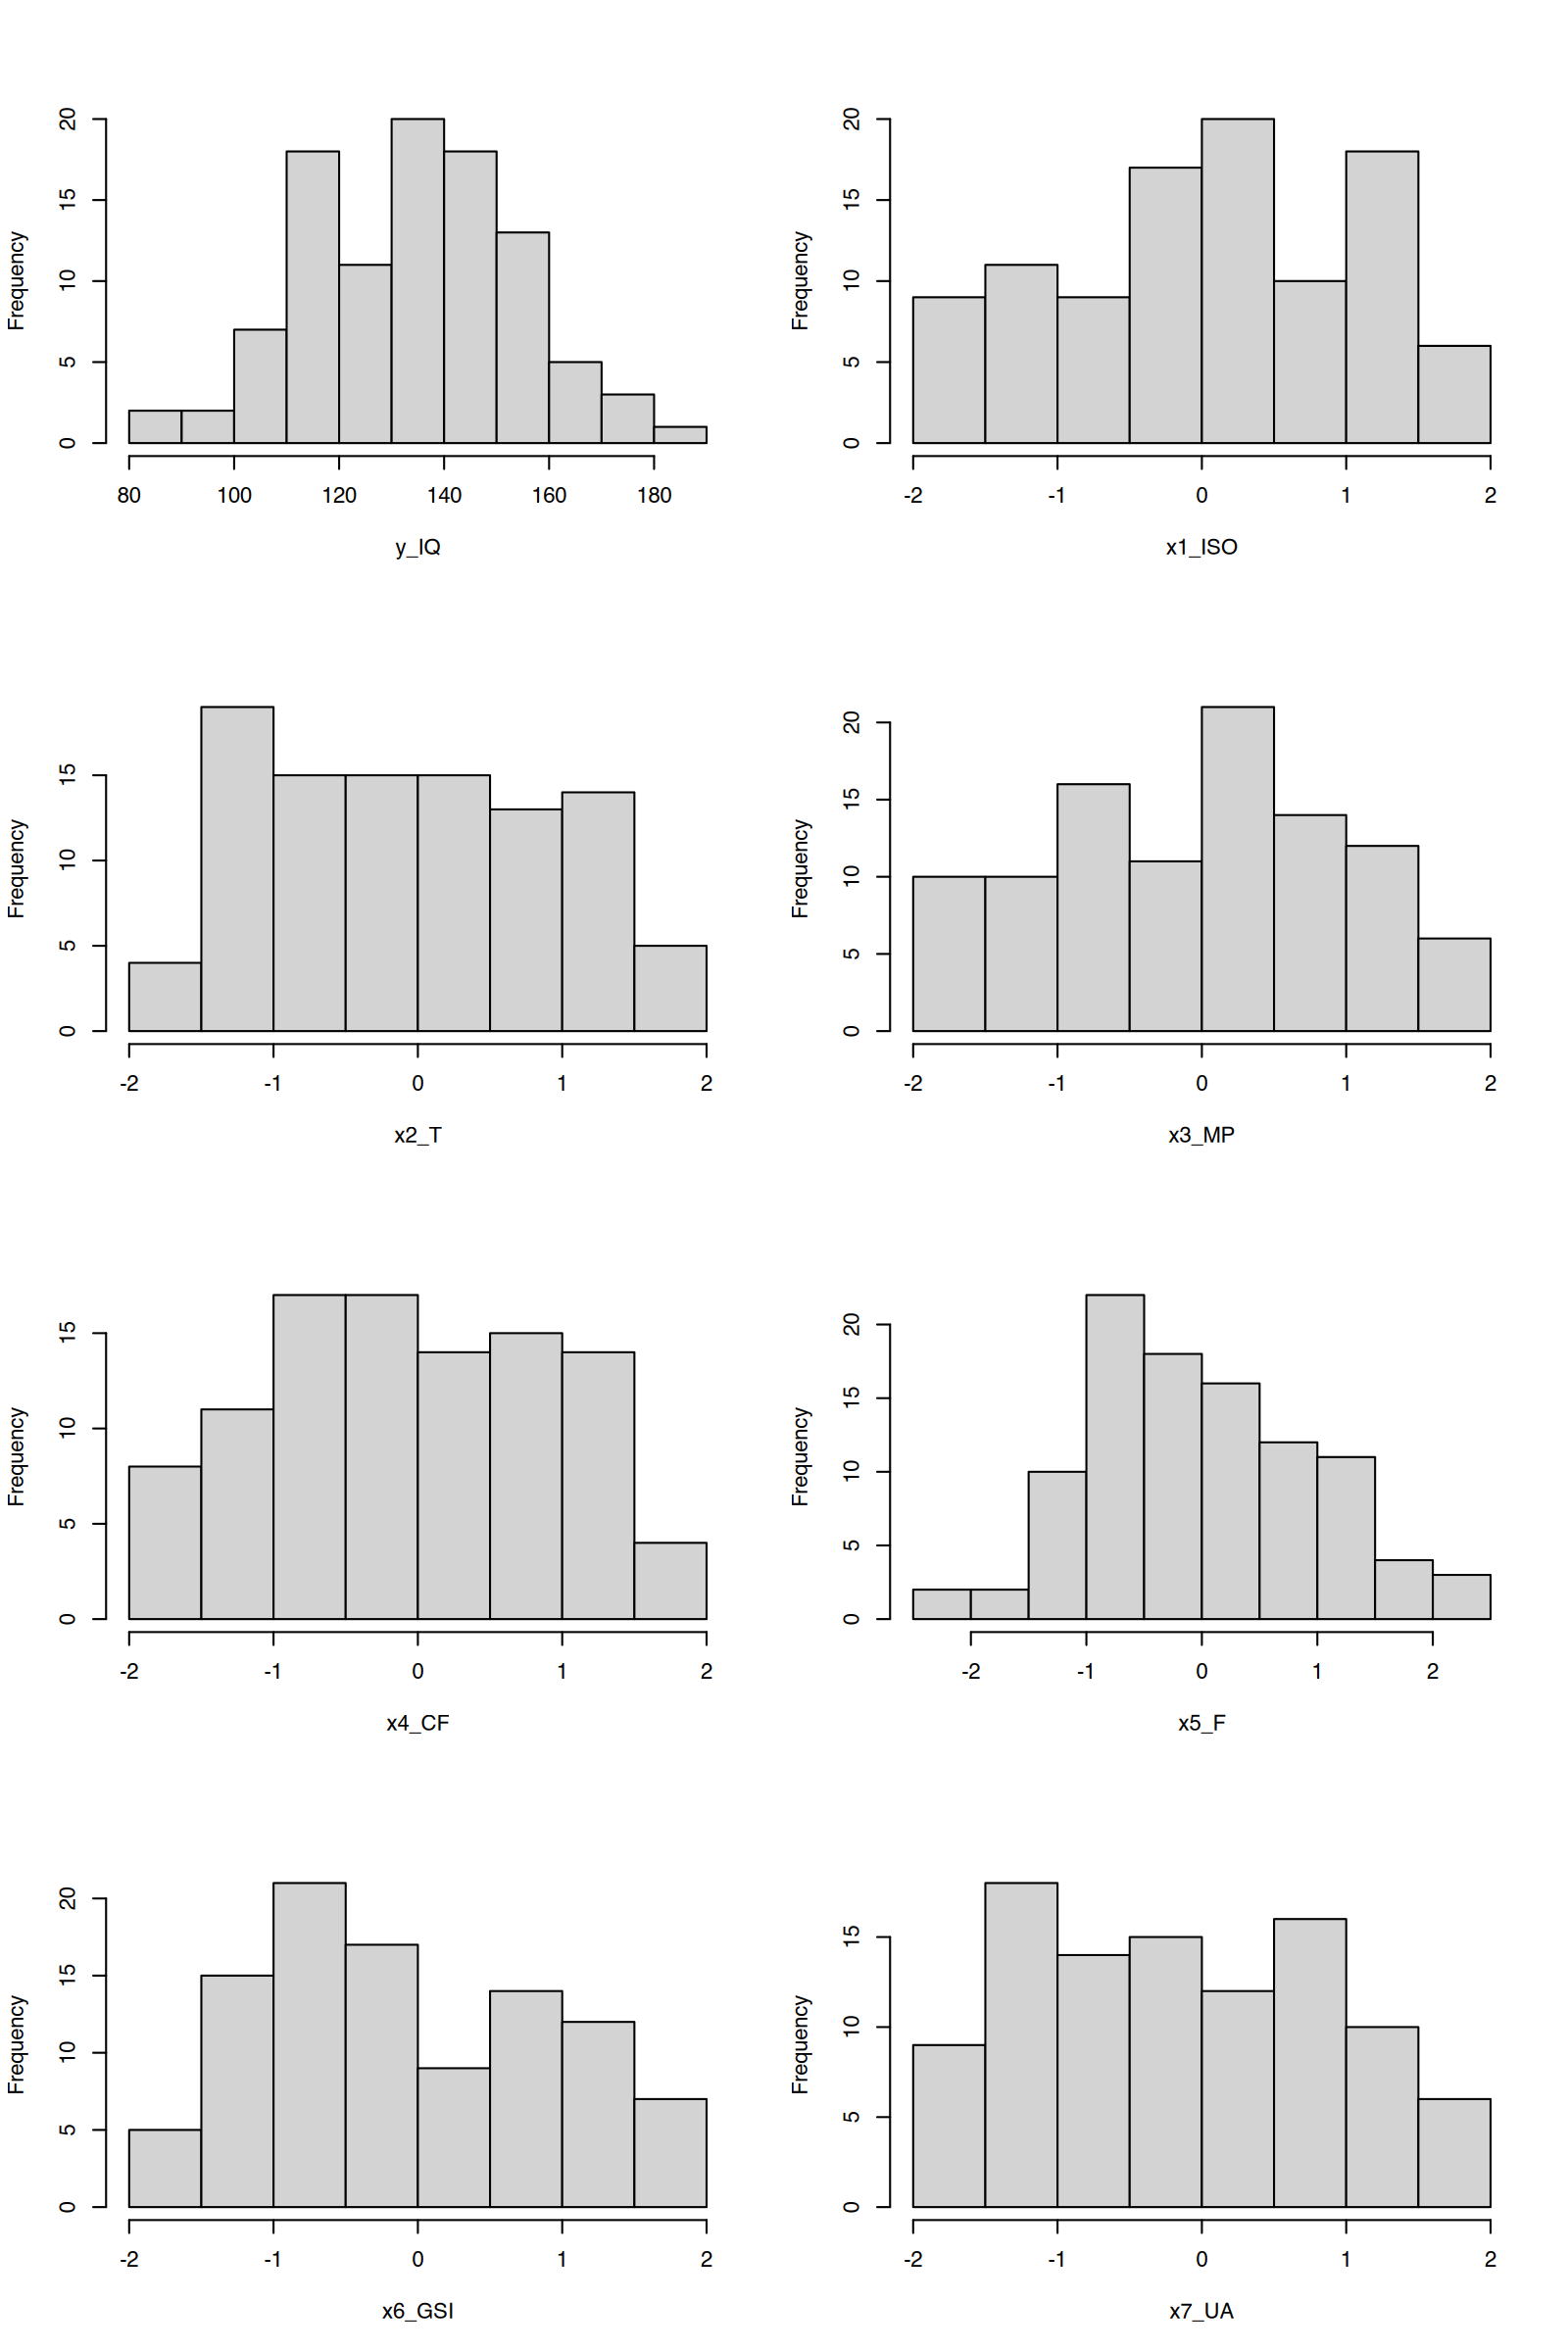
\includegraphics[width=0.88\linewidth]{figures/plottwists/hists.png}
\caption{histograms}
\end{figure}

Non si notano somiglianze a distribuzioni particolari per la maggior parte delle variabili, meno che per \texttt{\detokenize{y_IQ}} e \texttt{\detokenize{x5_F}}, che nonostante alcuni rilevanti scostamenti, sono approssimabili a distribuzioni normali.

Per verificare ciò è possibile analizzarne i Q-Q plots, grafici che confrontano i quantili dei dati campionari con quelli della distribuzione teorica supposta (normale: \texttt{\detokenize{qqnorm()}}).

Tale visualizzazione è accompagnata dai risultati del test d'ipotesi di Shapiro-Wilk ovvero:

\[
\begin{array}{ll}
H_0: \text{i dati provengono da} & \qquad\qquad H_A: \text{i dati non provengono da} \\
\phantom{H_0: }\text{una distribuzione normale} & \qquad\qquad \phantom{H_A: }\text{una distribuzione normale}
\end{array}
\]

Il test si effettua valutando la statistica-test:

\[
0 \underset{H_A}{\le} W = \frac{\left(\sum_{i=1}^n a_i x_{(i)}\right)^2}{\sum_{i=1}^n (x_i - \bar{x})^2} \underset{H_0}{\le} 1
\]

Scegliendo un livello di significatività $\alpha = 0.05$ (equivalentemente un livello di confidenza $1-\alpha = 0.95$), il criterio di scelta è:

\[
p = \mathbb{P}(T_n = W < t_n = w_{\text{oss}} \mid H_0) \space \underset{H_A}{\overset{H_0}{\gtrless}} \space \alpha = 0.05
\]

\begin{figure}[H]
\centering
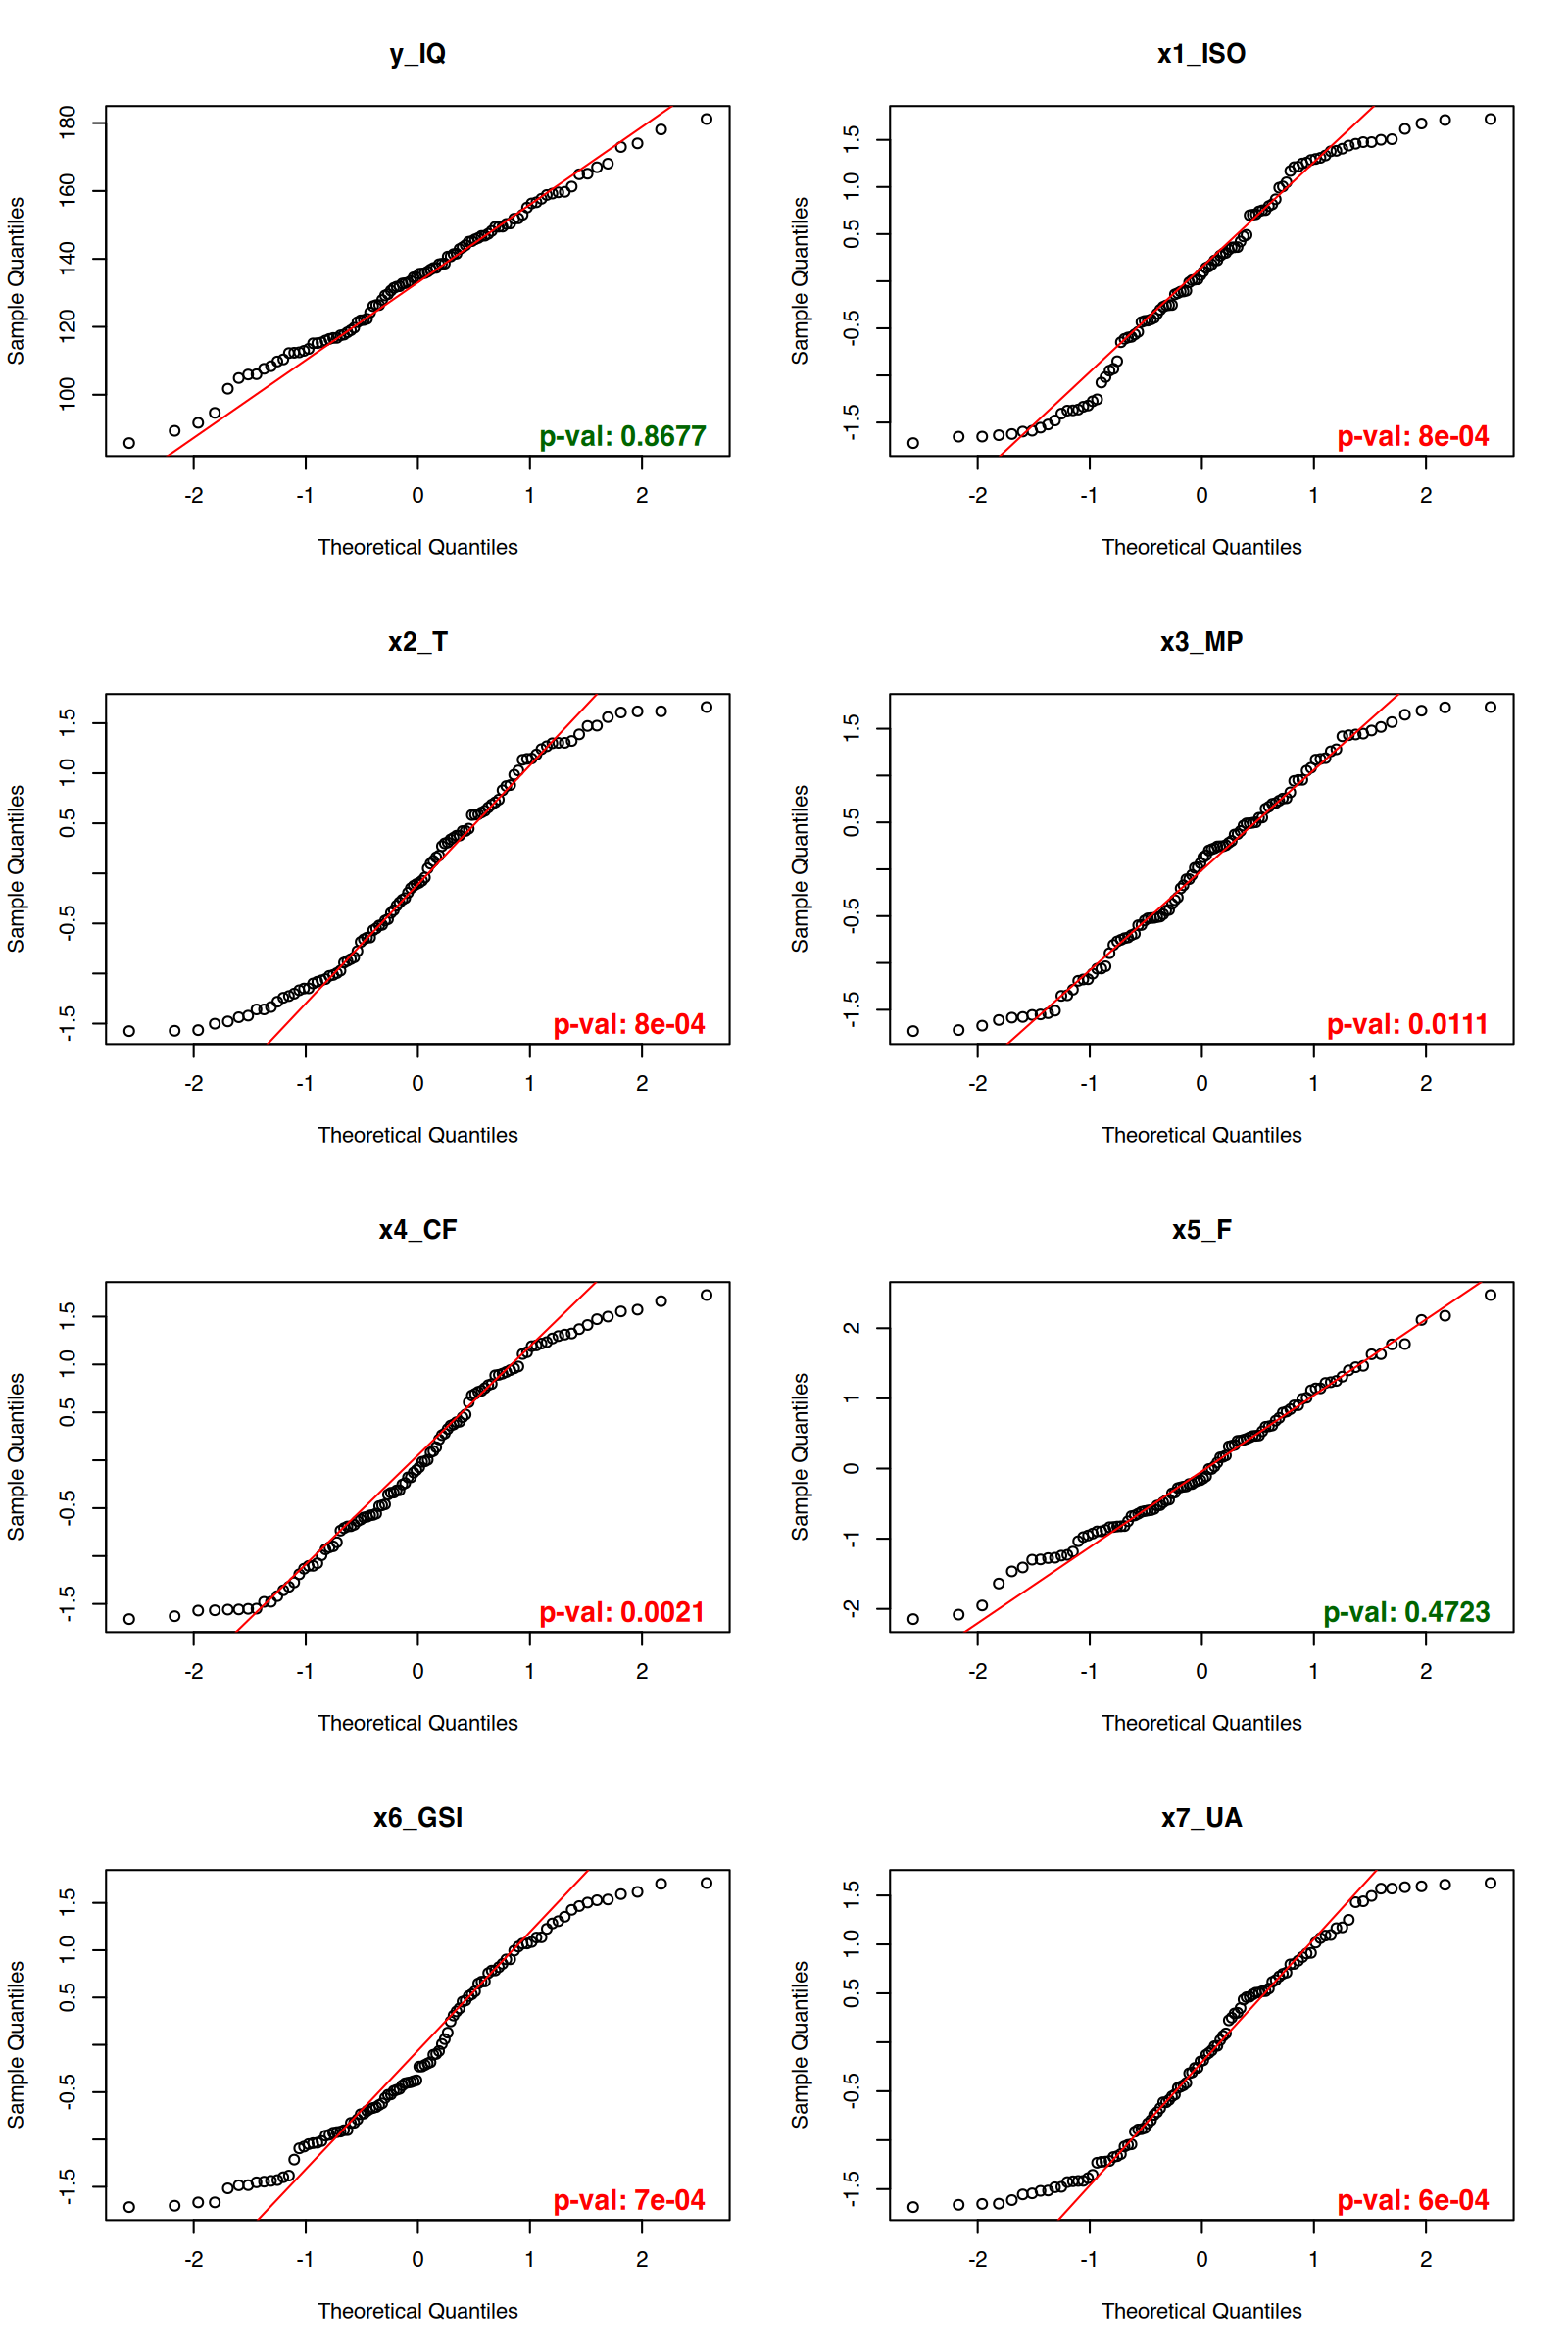
\includegraphics[width=0.88\linewidth]{figures/plottwists/qq_normals.png}
\caption{qq normals}
\end{figure}

Notiamo che nel caso di \texttt{\detokenize{y_IQ}} il p-value è 0.86, ovvero ipotizzando che la popolazione sia perfettamente normale, la probabilità di ottenere un campione con una distribuzione meno aderente a quella normale è dell'86\%.

Dato che il livello di significatività è 0.05, non possiamo rifiutare l'ipotesi nulla, di conseguenza possiamo assumere che i dati provengano da una distribuzione normale.

Ciò accade anche per la variabile \texttt{\detokenize{x5_F}}, che come visualizzato sul Q-Q plot segue con buona approssimazione la retta teorica \texttt{\detokenize{qqline()}}.

\subsection{1.3. Scatter Plot}
\label{sec:13-scatter-plot}

Un altro strumento utile per visualizzare la relazione tra variabili è lo scatter plot, che rappresenta i dati come punti in un piano cartesiano. Ognuna delle variabili è rappresentata su un asse, limitandosi solitamente a due variabili per grafico.

Per maggiore chiarezza visiva, abbiamo incluso due linee per ogni grafico, una rappresenta la regressione semplice (\texttt{\detokenize{lm(b ~ a)}}) e l'altra la regressione polinomiale di secondo grado (\texttt{\detokenize{lm(b ~ poly(a, 2, raw = TRUE))}}). In questa fase, sono utilizzate per meglio dirigere l'attenzione verso eventuali relazioni tra le variabili, che potrebbero altrimenti essere meno evidenti.

Partiamo dalla variabile dipendente \texttt{\detokenize{y_IQ}}, confrontandola con le variabili indipendenti.

\begin{figure}[H]
\centering
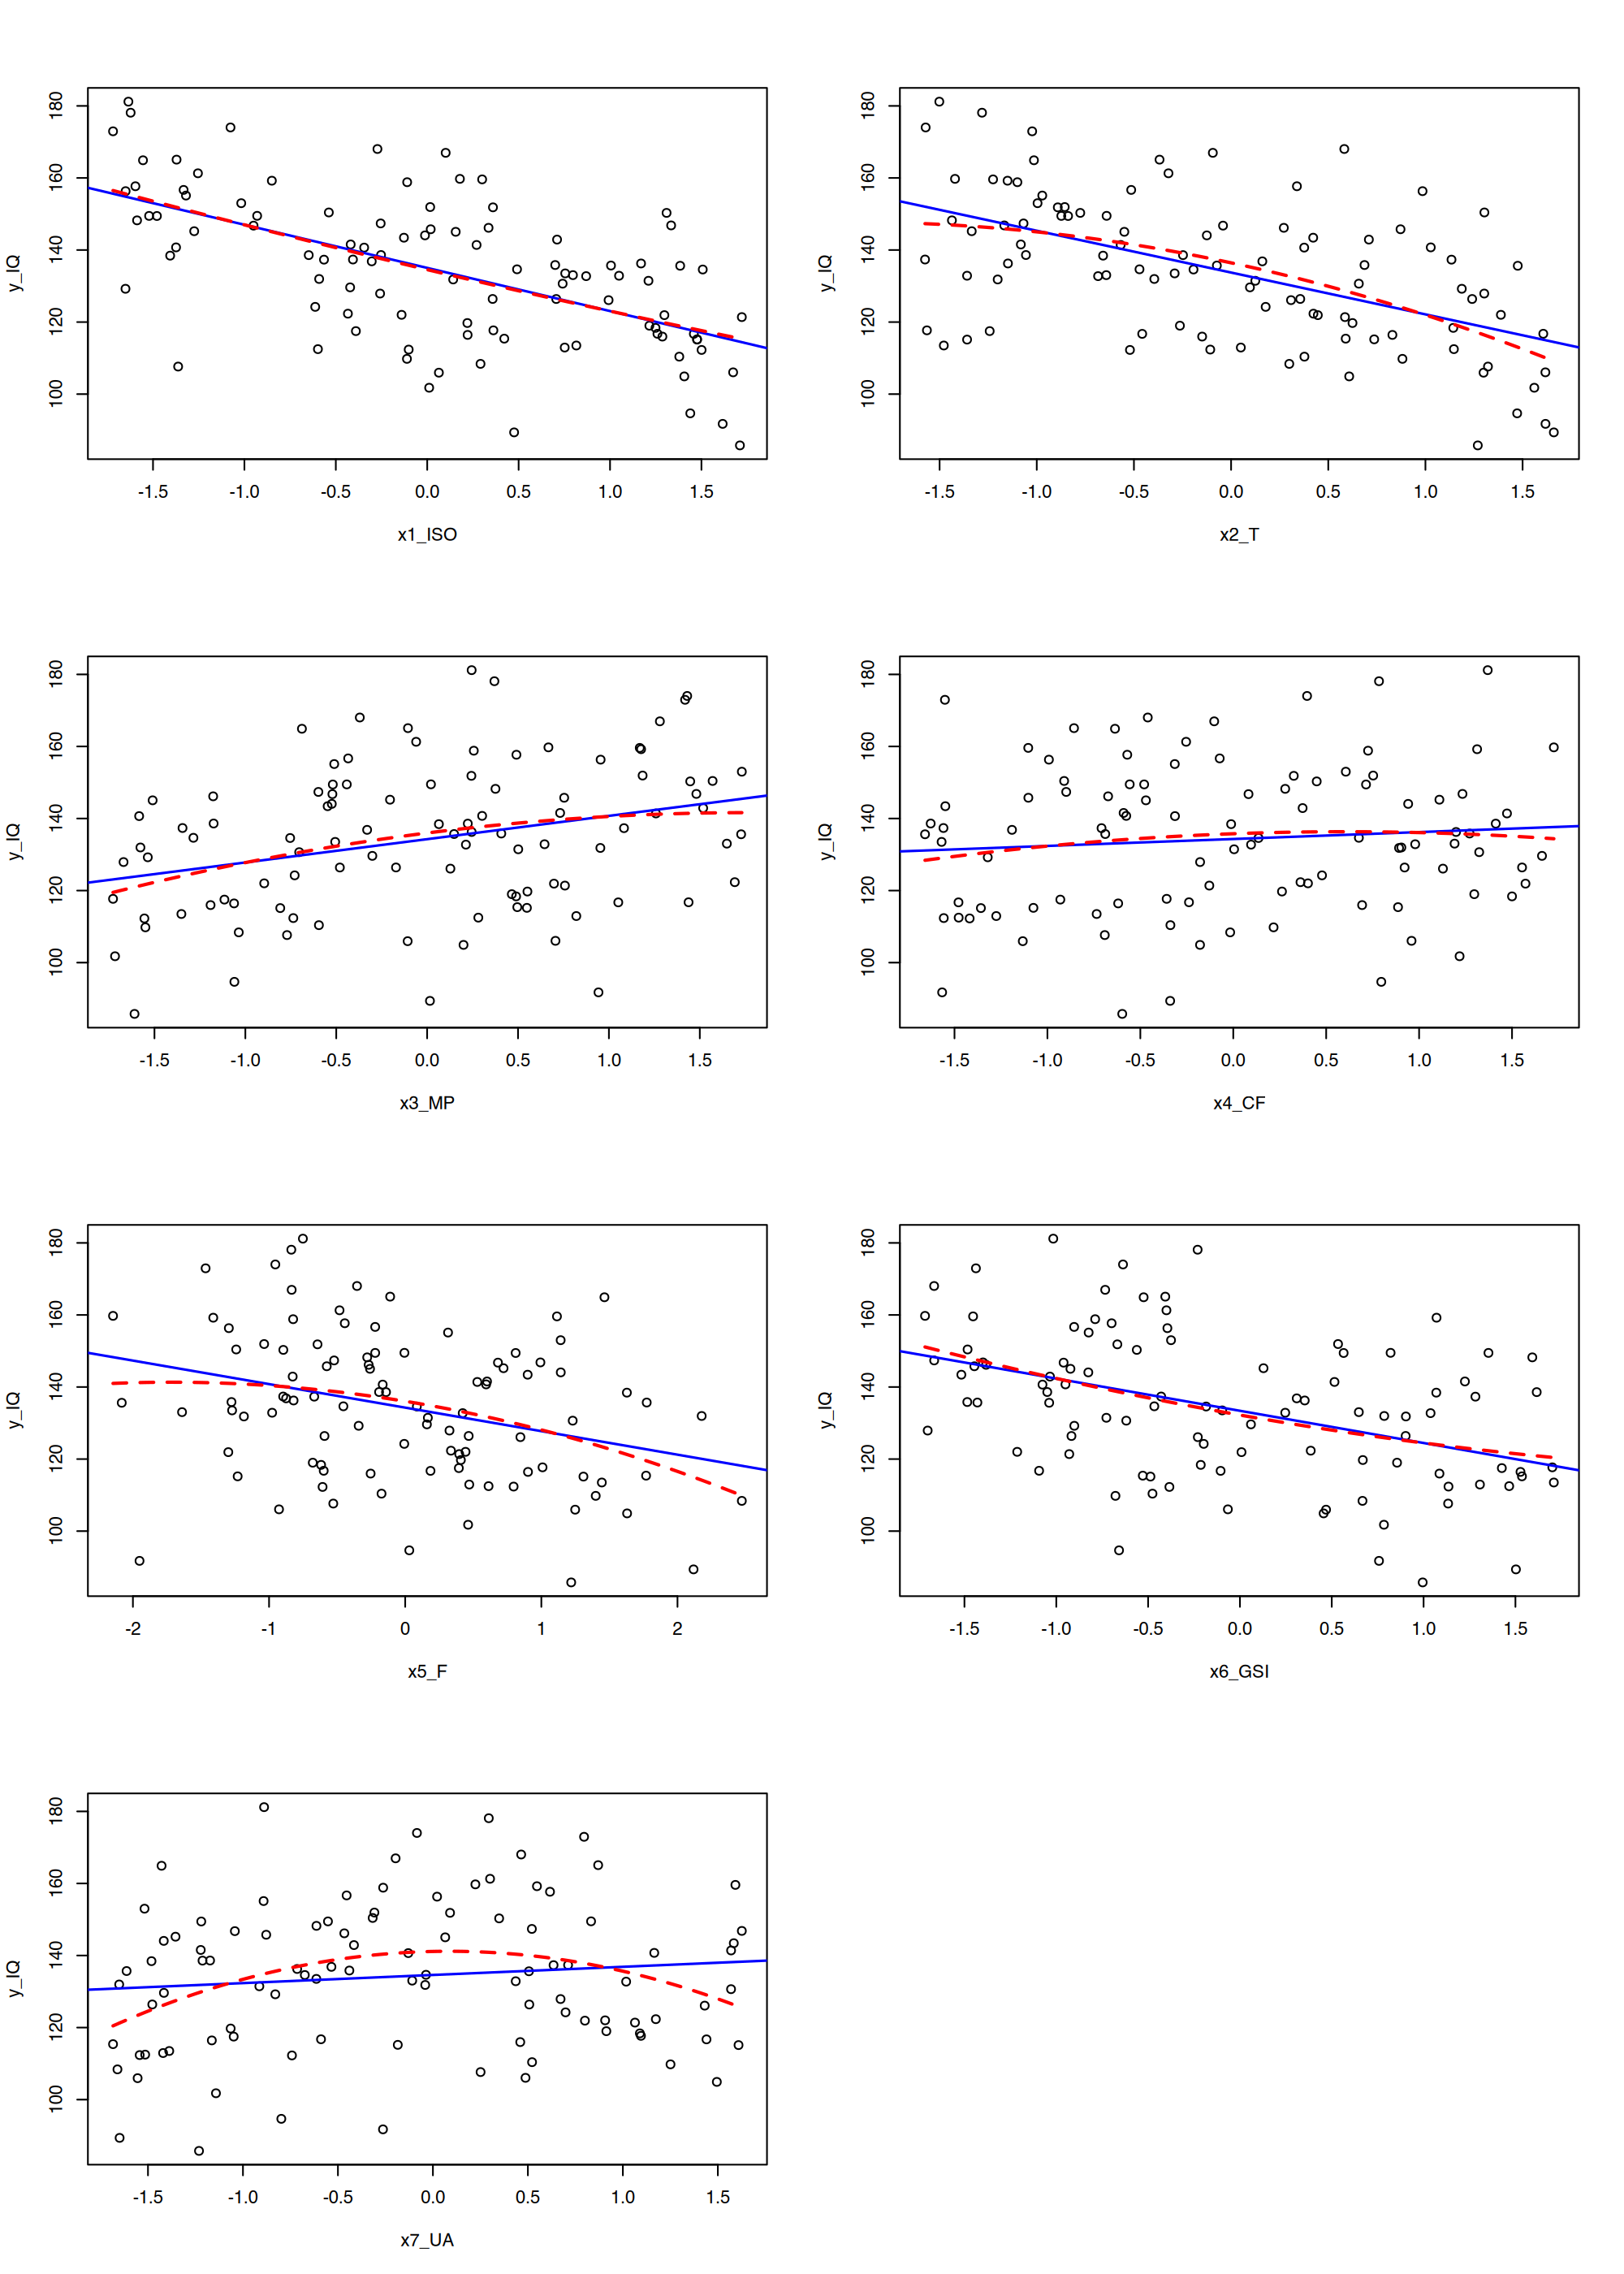
\includegraphics[width=0.88\linewidth]{figures/plottwists/scatters_y_vs_xs_lines.png}
\caption{scatter y vs xs lines}
\end{figure}

Possiamo già notare che, da un punto di vista lineare, \texttt{\detokenize{y_IQ}} sembra essere negativamente correlata con \texttt{\detokenize{x1_ISO}}, \texttt{\detokenize{x2_T}}, \texttt{\detokenize{x5_F}} e \texttt{\detokenize{x6_GSI}}. Mostra poi una relazione positiva con \texttt{\detokenize{x3_MP}}, e sembrerebbe non avere correlazione, se non molto debole, con \texttt{\detokenize{x4_CF}} e \texttt{\detokenize{x7_UA}}.

Una particolarità è che \texttt{\detokenize{x7_UA}} sembra avere una relazione quadratica molto evidente con \texttt{\detokenize{y_IQ}}, che non è invece visibile nella regressione lineare.

Osserviamo ora la relazione tra le variabili indipendenti.

\begin{figure}[H]
\centering
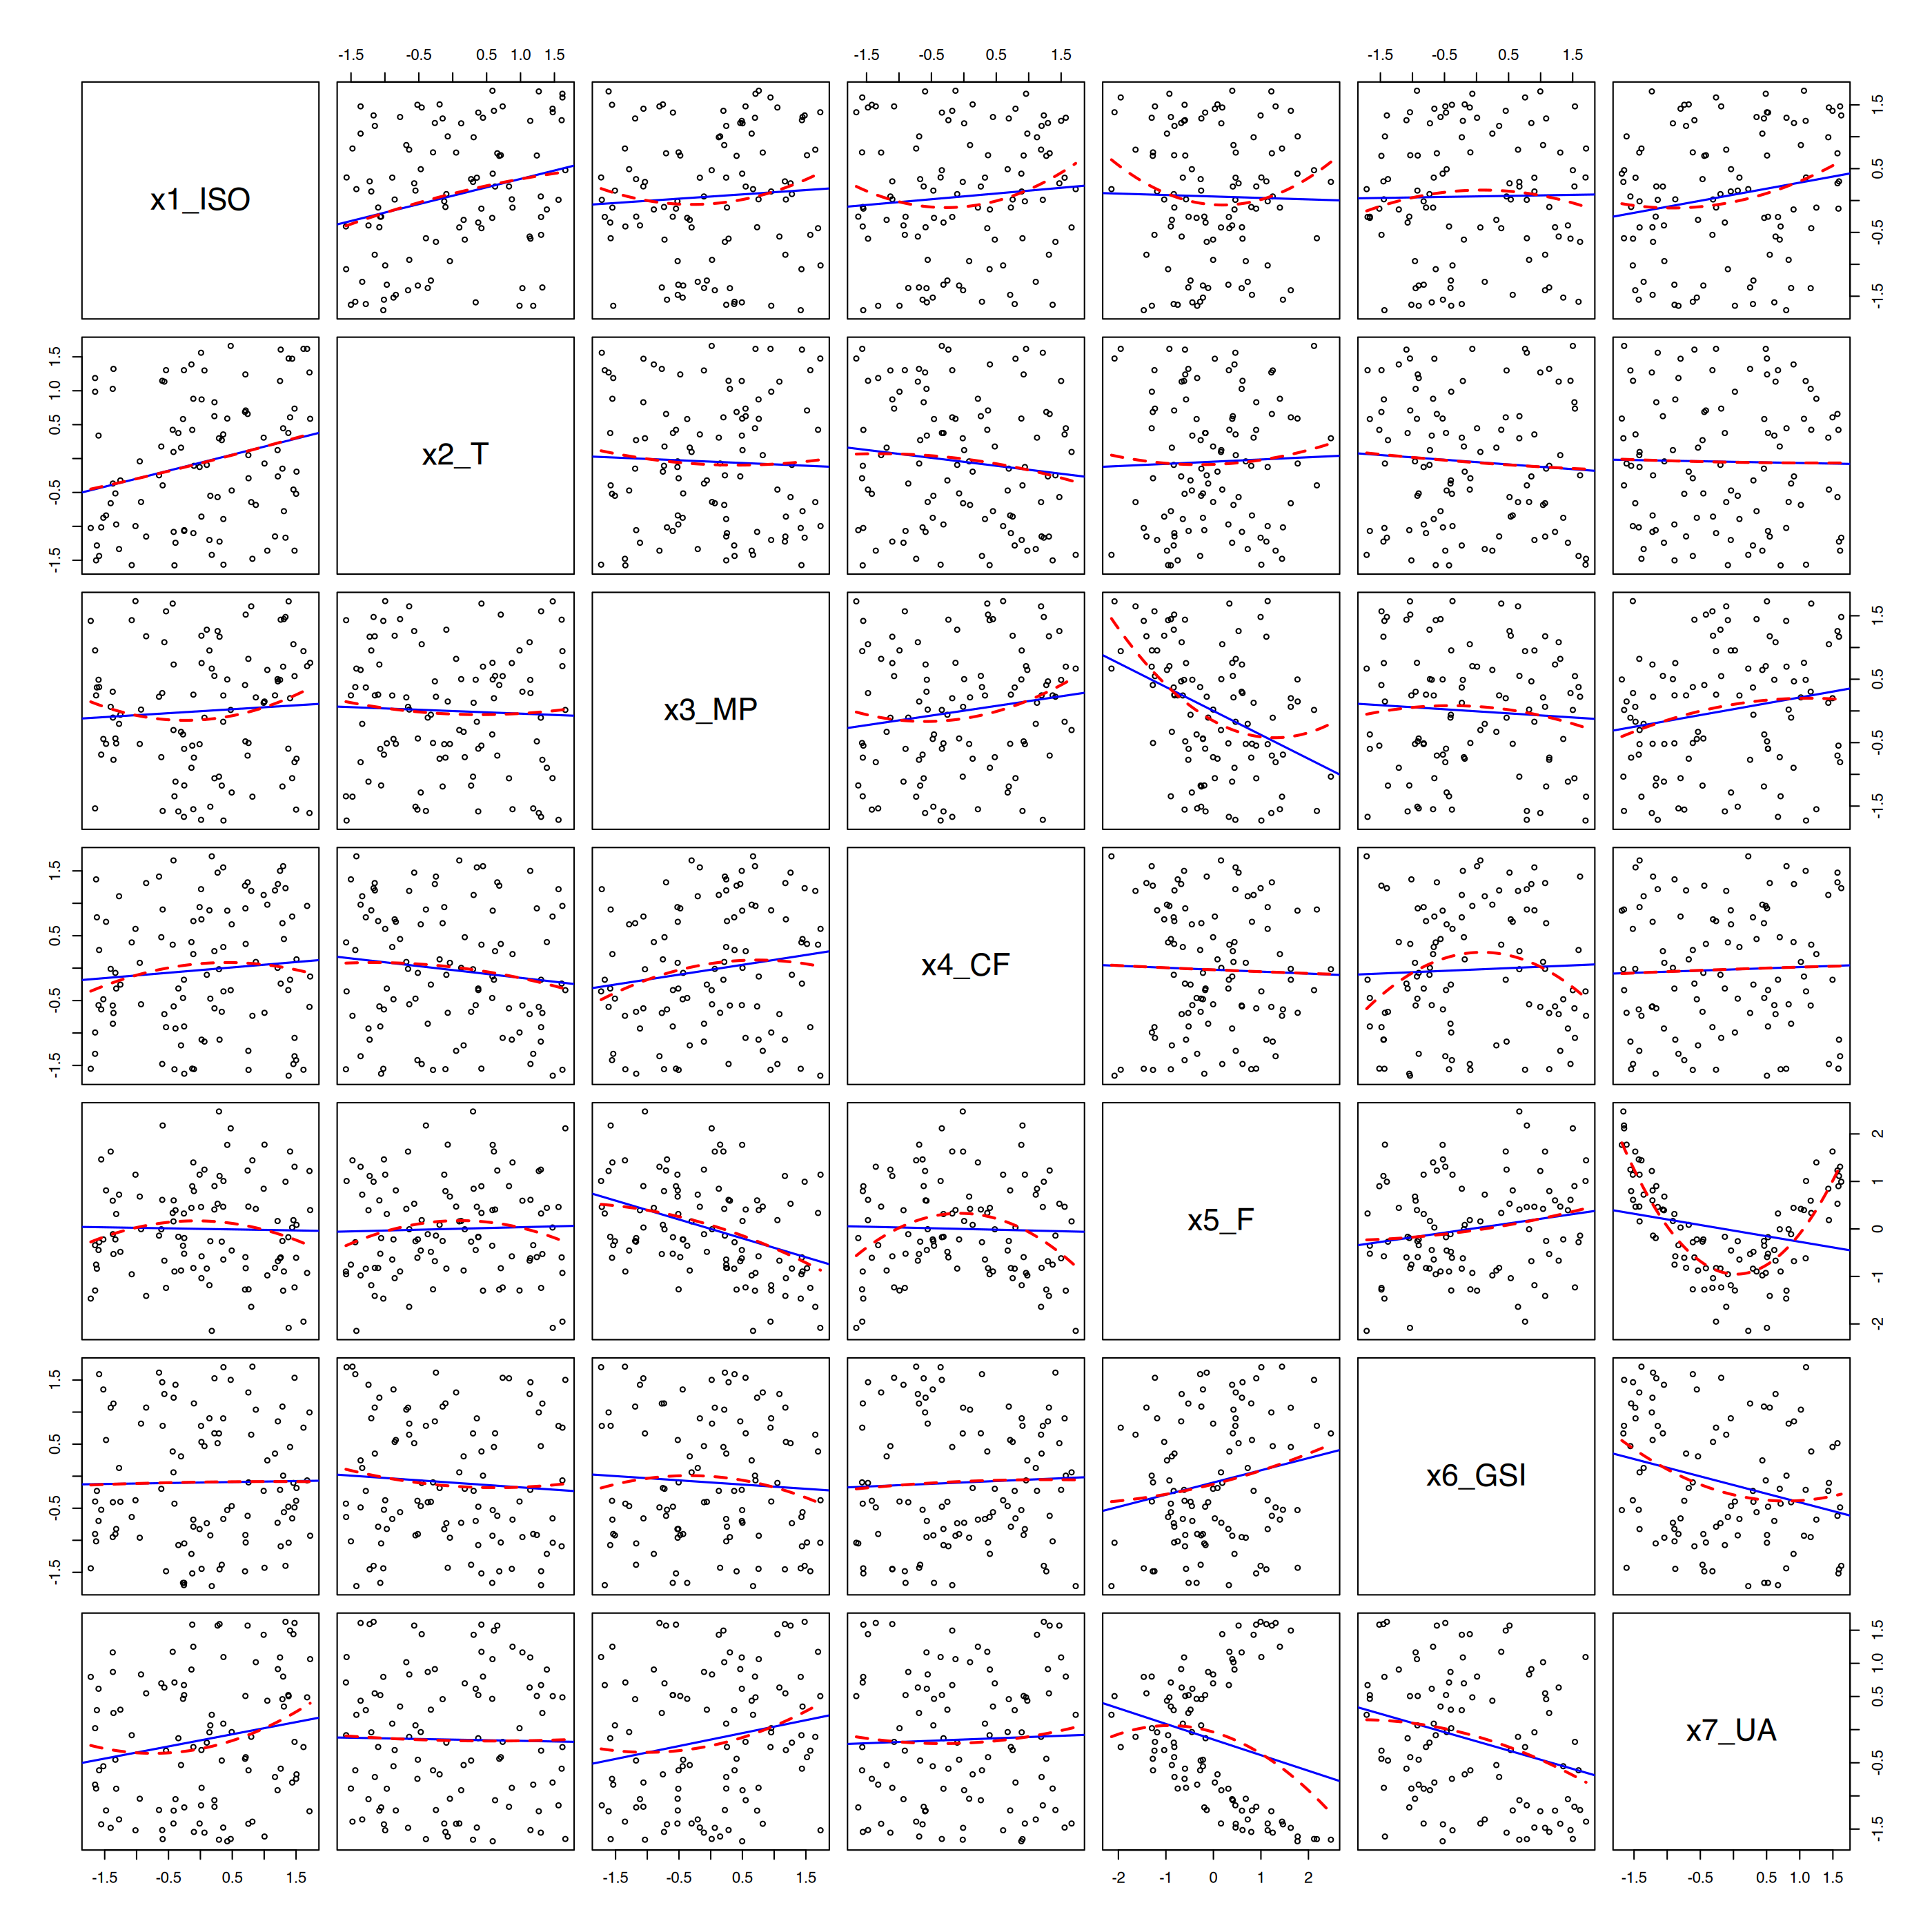
\includegraphics[width=0.88\linewidth]{figures/plottwists/scatters_all_lines.png}
\caption{scatter all lines}
\end{figure}

In questo caso, la maggior parte delle variabili non sembra avere correlazioni evidenti. L'eccezione più importante è quella di \texttt{\detokenize{x5_F}} e diverse altre variabili. Linearmente, \texttt{\detokenize{x5_F}} presenta una forte relazione con \texttt{\detokenize{x3_MP}} e, da un punto di vista quadratico, è in relazione con \texttt{\detokenize{x4_CF}}, e, in particolare, con \texttt{\detokenize{x7_UA}}.

Vorremmo riportare con più enfasi la relazione tra \texttt{\detokenize{x5_F}} e \texttt{\detokenize{x7_UA}}, che mostra un chiaro caso in cui l'assenza di correlazione non implica l'assenza di relazione tra le variabili. In questo caso, la relazione è chiaramente quadratica.

\begin{figure}[H]
\centering
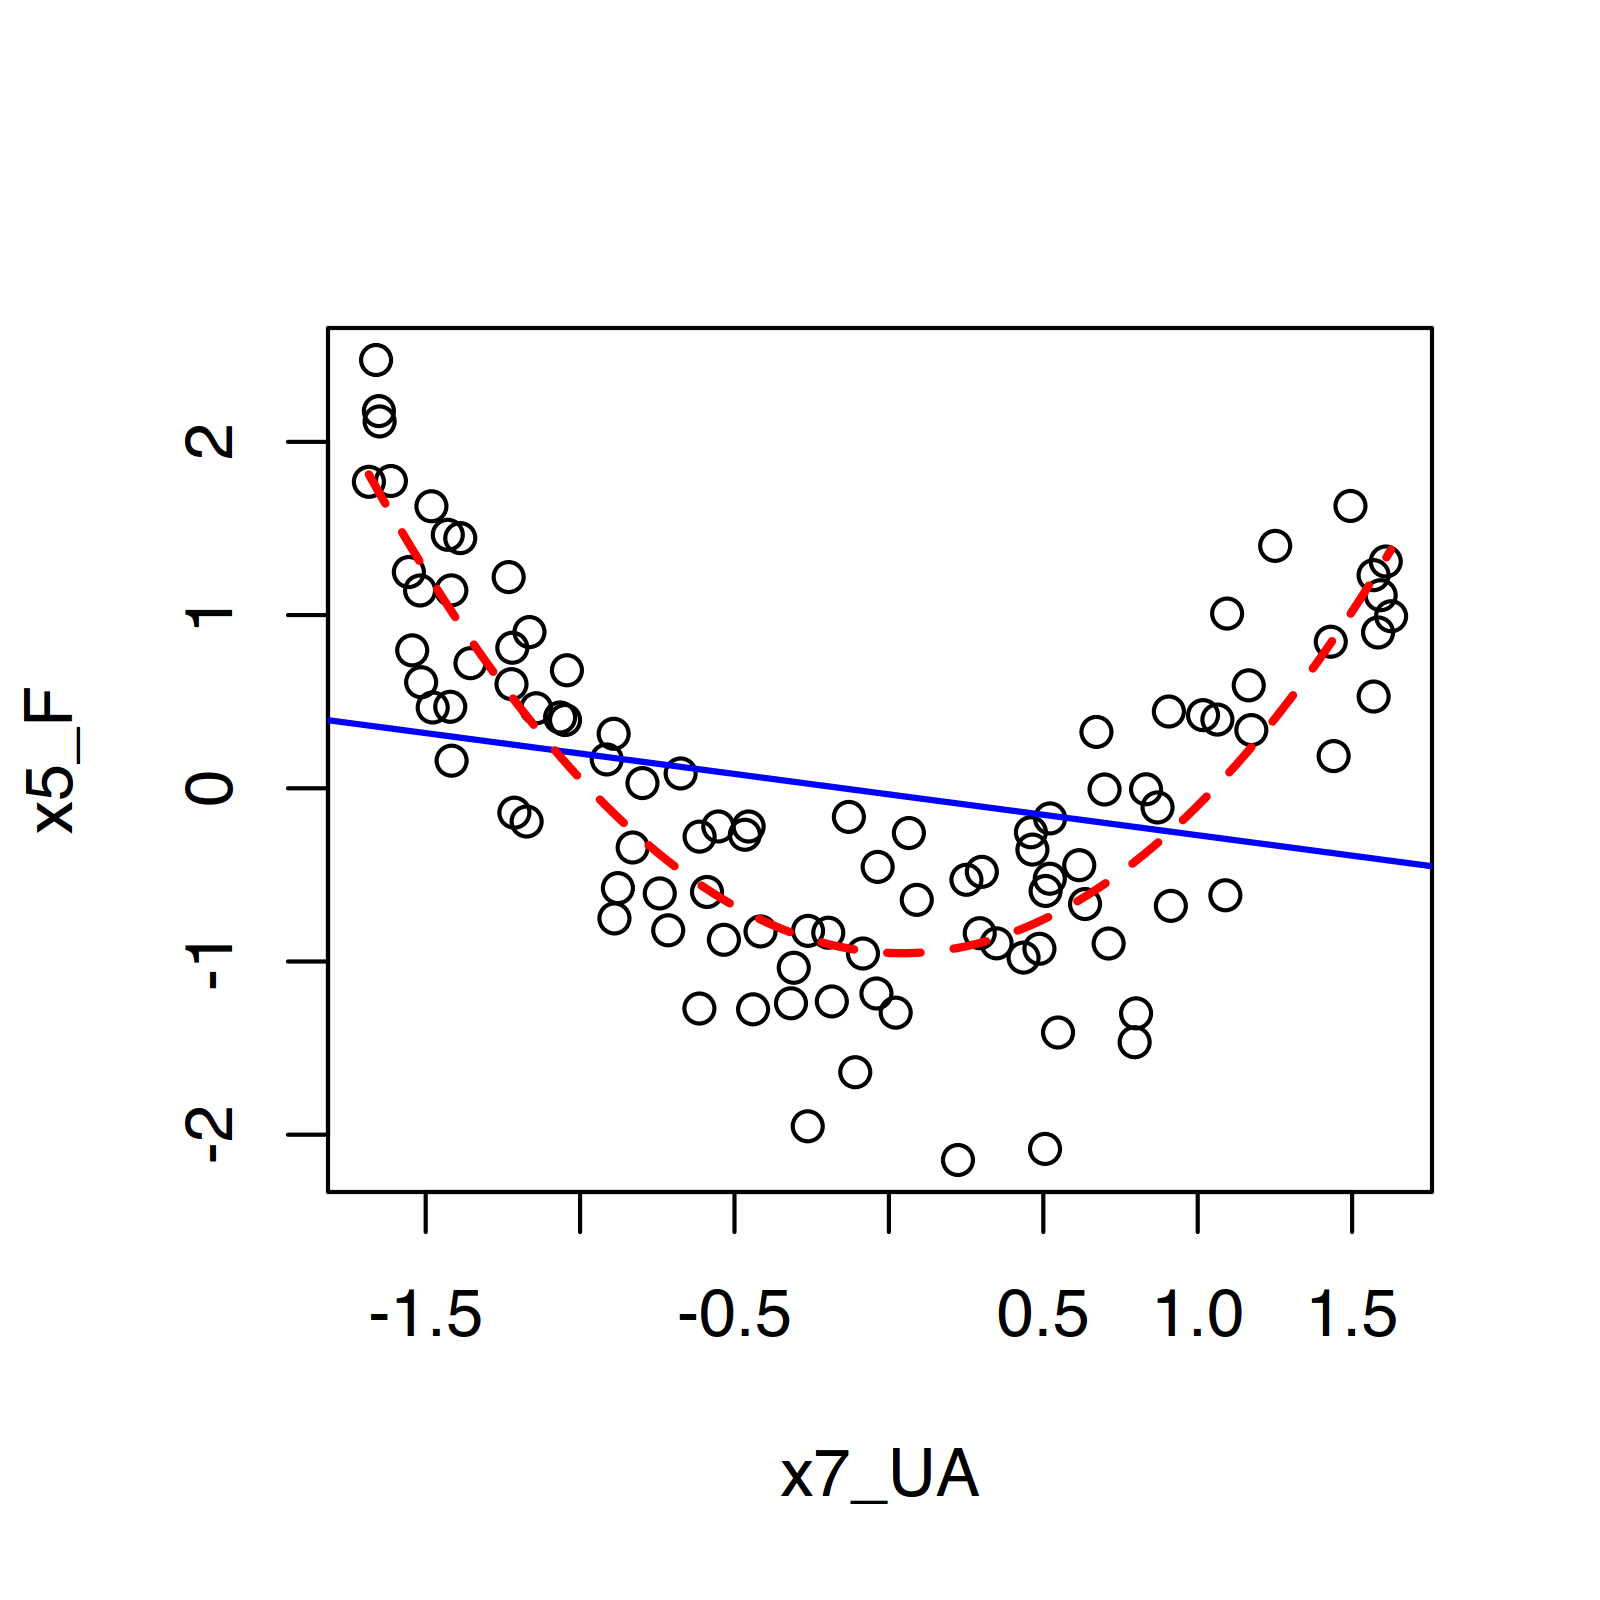
\includegraphics[width=0.40\linewidth]{figures/plottwists/x7_UA_vs_x5_F.png}
\caption{x7 UA vs x5 F}
\end{figure}

\subsection{1.4. Analisi di Correlazione}
\label{sec:14-analisi-di-correlazione}

Procediamo ora a valutare la correlazione tra le variabili, per ottenere informazioni più precise sulle relazioni tra di esse.

\begin{figure}[H]
\centering
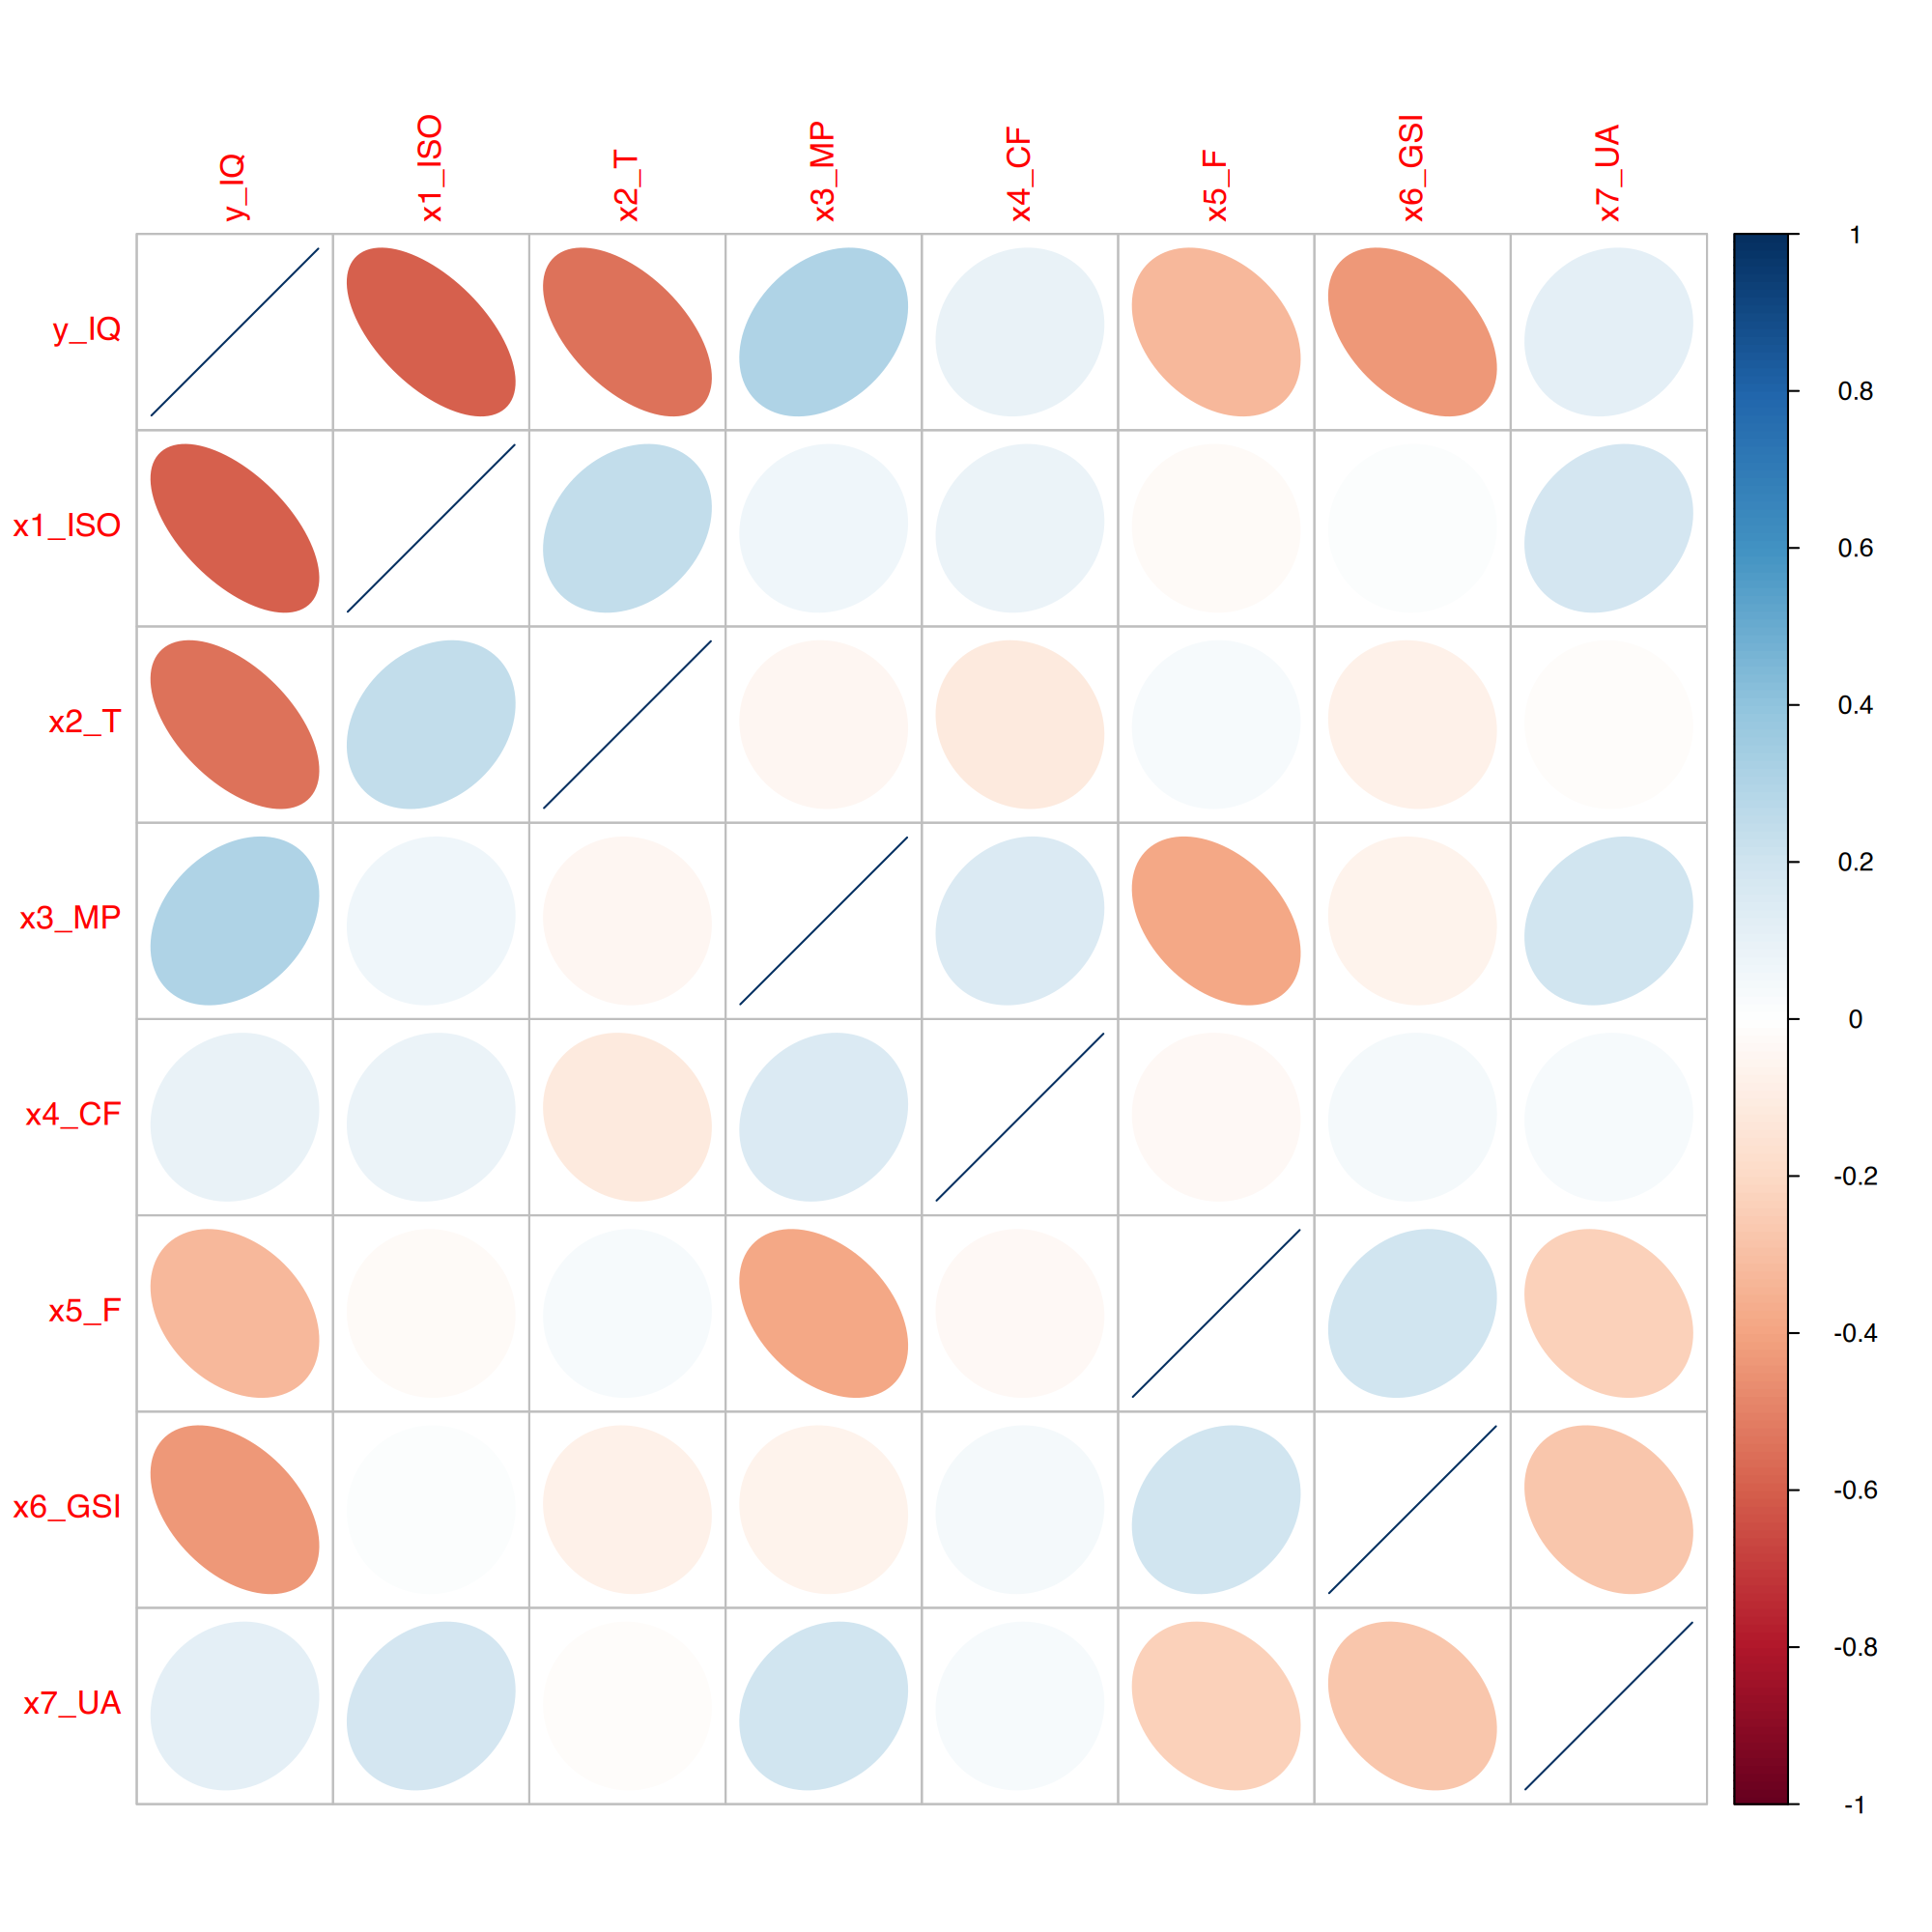
\includegraphics[width=0.80\linewidth]{figures/plottwists/corrplot.png}
\caption{corrplot}
\end{figure}

\begin{figure}[H]
\centering
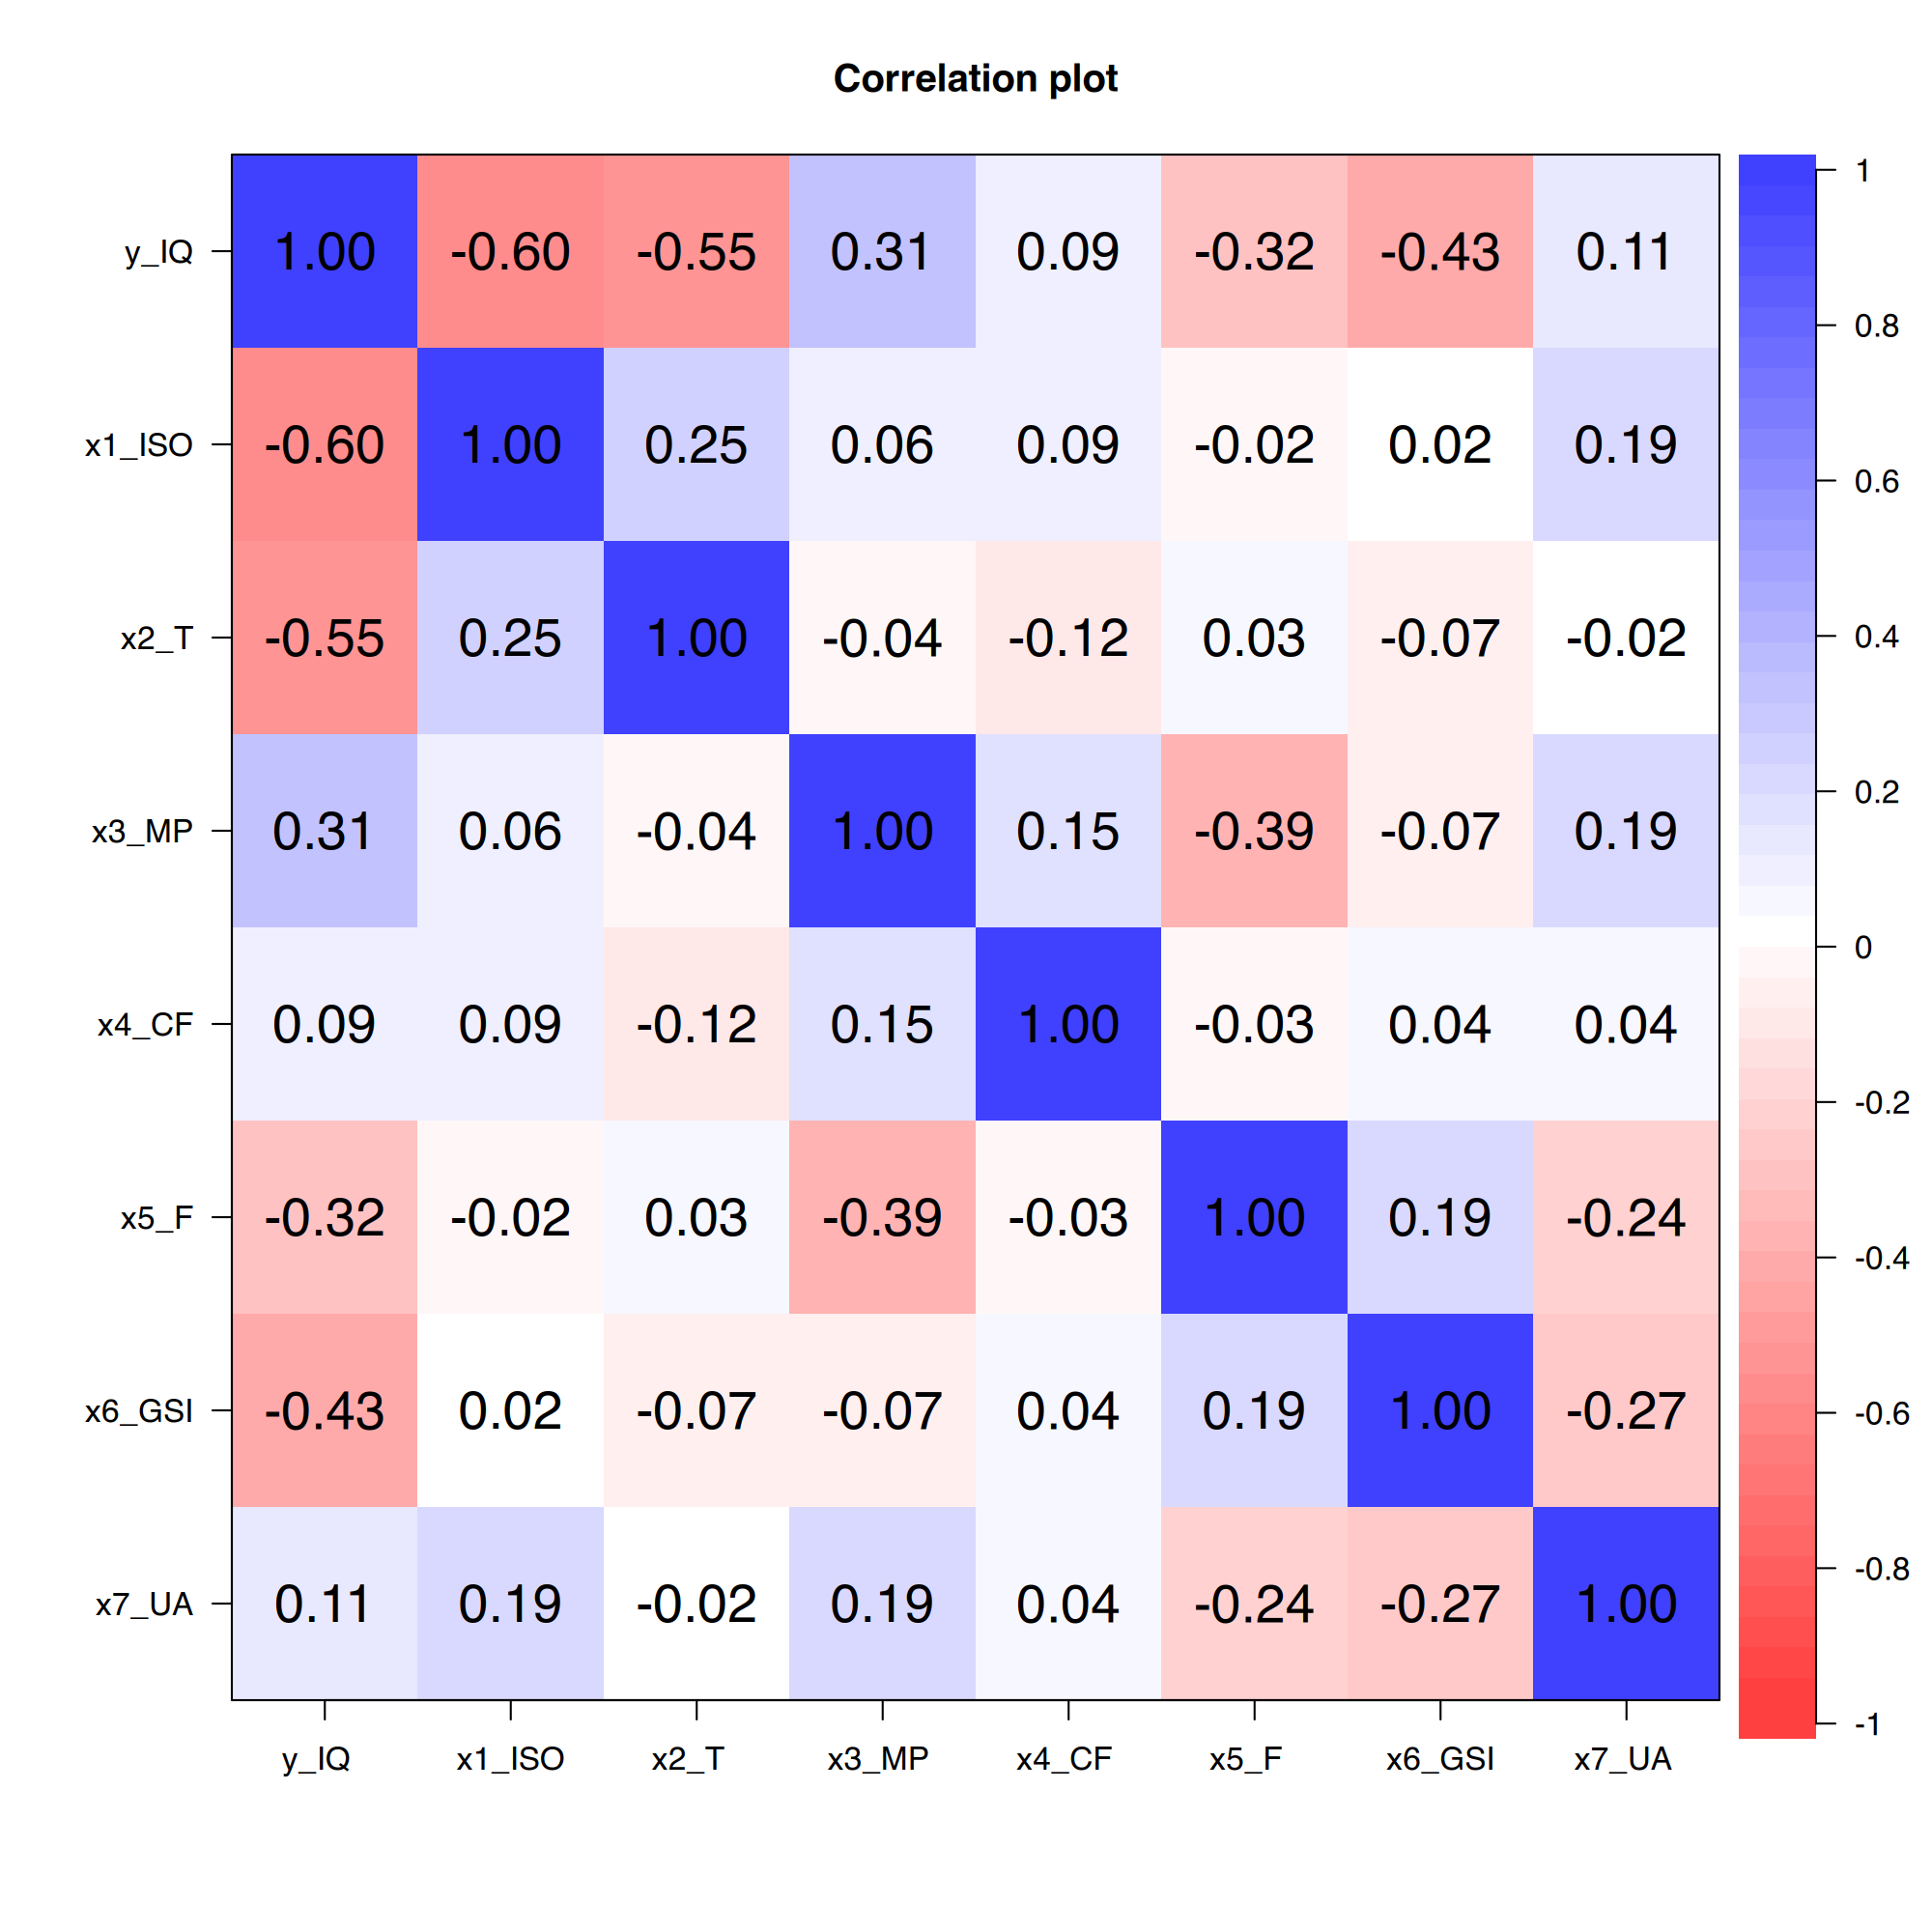
\includegraphics[width=0.80\linewidth]{figures/plottwists/corrplot_heatmap.png}
\caption{corrplot heatmap}
\end{figure}

Basandoci sulle indicazioni presentate durante il corso, possiamo interpretare i valori di correlazione secondo la seguente tabella:

\begin{table}[H]
\centering
\begin{tabular}{ll}
\toprule
Valore di |R| & Interpretazione \\
\midrule
|R| $\in$ [0.9, 1.0] & Correlazione "molto alta" \\
|R| $\in$ [0.7, 0.9) & Correlazione "alta" \\
|R| $\in$ [0.5, 0.7) & Correlazione "moderata" \\
|R| $\in$ [0.2, 0.5) & Correlazione "bassa" \\
|R| $\in$ [0, 0.2) & Correlazione "trascurabile" \\
\bottomrule
\end{tabular}
\end{table}

Questi grafici sembrano confermare le ipotesi fatte in precedenza. Non ci troviamo in presenza di correlazioni particolarmente forti. Esplorando i legami tra \texttt{\detokenize{y_IQ}} e le variabili indipendenti, si può notare che con le variabili \texttt{\detokenize{x1_ISO}} e \texttt{\detokenize{x2_T}} è presente una moderata correlazione negativa. Anche con \texttt{\detokenize{x5_F}} e \texttt{\detokenize{x6_GSI}} notiamo una correlazione negativa, ma bassa. Infine, con \texttt{\detokenize{x3_MP}} c'è una bassa correlazione positiva. Tutte le altre variabili sono correlate con \texttt{\detokenize{y_IQ}} in maniera trascurabile.

Tra le variabili indipendenti, spicca la correlazione negativa tra \texttt{\detokenize{x5_F}} e \texttt{\detokenize{x3_MP}}, che avevamo già notato in precedenza, e risulta presente anche una correlazione negativa tra \texttt{\detokenize{x5_F}} e \texttt{\detokenize{x7_UA}} (oltre alla loro relazione polinomiale), e tra \texttt{\detokenize{x6_GSI}} e \texttt{\detokenize{x7_UA}}, che non erano state menzionate prima.

In ogni caso, le correlazioni tra le variabili indipendenti menzionate sono basse, e tutte le altre risultano essere trascurabili. Ci aspettiamo quindi di vedere pochi termini multipli nella fase finale.

\section{2. Regressione}
\label{sec:2-regressione}

Nella presente sezione utilizzeremo un'altra serie di strumenti per la ricerca di una superficie di risposta, ovvero un modello che approssimi la realtà e ci permetta di stimare i legami tra la grandezza di interesse \texttt{\detokenize{y_IQ}}, e le variabili indipendenti, che prendono il nome di regressori.

Uno degli indici di "bontà" del modello è il coefficiente di determinazione $R^2$:

\[
0 \underset{\text{useless}}{\le} R^2 = \frac{SQR}{SQTOT} \underset{\text{ideal}}{\le} 1
\]

Esso misura la quota della variabilità totale ($SQTOT$) di \texttt{\detokenize{y_IQ}} spiegata dal modello di regressione ($SQR$), dove:

\[
\overset{SQTOT}{\sum_{i=1}^{n} (Y_i - \bar{Y})^2} = \overset{SQR}{\sum_{i=1}^{n} (\hat{Y}_i - \bar{Y})^2} + \overset{SQE}{\sum_{i=1}^{n} (Y_i - \hat{Y}_i)^2}
\]

In questa formula, detta \emph{Teorema di decomposizione della devianza}, $Y$ rappresenta i valori osservati di \texttt{\detokenize{y_IQ}}, $\hat{Y}$ rappresenta i valori stimati dal modello, e $\bar{Y}$ rappresenta la media dei valori osservati di \texttt{\detokenize{y_IQ}}.

\subsection{2.1. Analisi di Modelli Lineari}
\label{sec:21-analisi-di-modelli-lineari}

I modelli considerati in questa fase sono definiti da parametri lineari, cioè sono nella forma:

\[
Y = \beta_0 + \beta_1 x_1 + \dots + \beta_p x_p + \varepsilon
\]

Nel nostro caso la stima viene effettuata tramite \texttt{\detokenize{lm()}}, che applica il metodo dei minimi quadrati. I coefficienti vengono quindi scelti in modo da minimizzare la somma dei quadrati dei residui:

\[
SQE = \sum_{i=1}^{n}(Y_i - \hat{Y}_i)^2
\]

Per ogni modello osserviamo sia il test globale F, che verifica se il modello nel suo complesso spiega una quota significativa della variabilità di \texttt{\detokenize{y_IQ}}, sia i test t sui singoli coefficienti.

\[
\begin{aligned}
\text{Test globale } F:\quad
& H_0: \beta_1 = \dots = \beta_p = 0,\quad
  H_A: \text{almeno un } \beta_j \neq 0\\
& F = \frac{MSQR}{MSQE}
    = \displaystyle{\frac{\frac{SQR}{p}}{\frac{SQE}{n-(p+1)}}}\\[0.6em]
\text{Test } t \text{ sui coefficienti}:\quad
& H_0: \beta_j = 0,\quad H_A: \beta_j \neq 0\\
& t_j = \displaystyle{\frac{\hat{\beta}_j}{\text{SE}(\hat{\beta}_j)}}
\end{aligned}
\]

Usiamo come riferimento un livello di significatività $\alpha = 0.05$: un p-value inferiore a tale soglia suggerisce che il contributo del regressore sia statisticamente significativo, a parità degli altri regressori presenti nel modello.

Pr(\textgreater{}|t|) indica il p-value del test t, mentre il p-value del test F è riportato in fondo al summary del modello.

\subsubsection{2.1.1. Classe 0: Modelli Lineari semplici}
\label{sec:211-classe-0-modelli-lineari-semplici}

Una prima ipotesi si può fare partendo da un modello che considera come regressori tutte le variabili indipendenti in maniera lineare.

\begin{lstlisting}[style=rconsole,caption={fit0}]
Residuals:
     Min       1Q   Median       3Q      Max
-16.4151  -6.0083  -0.0448   5.3063  23.9197

Coefficients:
             Estimate Std. Error t value Pr(>|t|)
(Intercept) 133.70383    0.87116 153.478  < 2e-16 ***
x1_ISO      -10.19229    0.88968 -11.456  < 2e-16 ***
x2_T         -9.08574    0.92760  -9.795 6.17e-16 ***
x3_MP         4.83753    0.96164   5.030 2.41e-06 ***
x4_CF         1.31206    0.89342   1.469  0.14536
x5_F         -2.95490    0.94569  -3.125  0.00238 **
x6_GSI       -8.55331    0.90959  -9.403 4.11e-15 ***
x7_UA         0.08169    0.92564   0.088  0.92987
---
Signif. codes:  0 '***' 0.001 '**' 0.01 '*' 0.05 '.' 0.1 ' ' 1

Residual standard error: 8.442 on 92 degrees of freedom
Multiple R-squared:  0.8408,    Adjusted R-squared:  0.8287
F-statistic: 69.43 on 7 and 92 DF,  p-value: < 2.2e-16
\end{lstlisting}

Il modello \texttt{\detokenize{fit0}} mostra già un ottimo p-value per il test globale F e coefficiente di determinazione $R^2$. Per il test t risultano poco significativi i regressori \texttt{\detokenize{x4_CF}} e \texttt{\detokenize{x7_UA}}, che andremo a rimuovere uno per volta nei due fit successivi, \texttt{\detokenize{fit1}} e \texttt{\detokenize{fit2}}, per valutare se la loro rimozione comporti un miglioramento del modello. Durante questa operazione notiamo una crescita dell'F-statistic, che suggerisce un miglioramento del modello, ma anche una crescita dell'errore standard residuo ed una lieve decrescita dell'$R^2$ dopo la seconda rimozione.

\subsubsection{2.1.2. Classe 00: Modelli con interazioni a due a due}
\label{sec:212-classe-00-modelli-con-interazioni-a-due-a-due}

Una seconda ipotesi consiste nell'aggiungere tutte le interazioni a due a due tra i regressori (\texttt{\detokenize{.^2}}). In questo modo il modello può descrivere situazioni in cui l'effetto di una variabile su \texttt{\detokenize{y_IQ}} dipende dal valore assunto da un'altra variabile.

\begin{lstlisting}[style=rconsole,caption={fit00}]
Residuals:
    Min      1Q  Median      3Q     Max
-16.567  -4.634  -0.109   4.933  23.722

Coefficients:
               Estimate Std. Error t value Pr(>|t|)
(Intercept)   133.89240    1.18604 112.890  < 2e-16 ***
x1_ISO         -9.53103    1.19481  -7.977 1.84e-11 ***
x2_T          -10.47134    1.28538  -8.146 8.95e-12 ***
x3_MP           3.99934    1.23660   3.234  0.00185 **
x4_CF           1.98511    1.29976   1.527  0.13113
x5_F           -2.49288    1.37656  -1.811  0.07438 .
x6_GSI         -8.46570    1.12739  -7.509 1.36e-10 ***
x7_UA          -0.04251    1.36524  -0.031  0.97525
x1_ISO:x2_T     0.35585    1.10511   0.322  0.74840
x1_ISO:x3_MP   -0.18932    1.33046  -0.142  0.88725
x1_ISO:x4_CF    0.75621    1.35418   0.558  0.57831
x1_ISO:x5_F     0.90324    1.32815   0.680  0.49867
x1_ISO:x6_GSI  -0.33701    1.17166  -0.288  0.77446
x1_ISO:x7_UA   -1.41419    1.37966  -1.025  0.30883
x2_T:x3_MP      0.25969    1.27341   0.204  0.83899
x2_T:x4_CF     -1.79419    1.30295  -1.377  0.17283
x2_T:x5_F      -1.58614    1.44128  -1.101  0.27483
x2_T:x6_GSI     0.39205    1.22269   0.321  0.74942
x2_T:x7_UA      0.76962    1.30911   0.588  0.55847
x3_MP:x4_CF    -2.29538    1.34869  -1.702  0.09314 .
x3_MP:x5_F     -0.01491    1.22538  -0.012  0.99033
x3_MP:x6_GSI    0.48022    1.31550   0.365  0.71616
x3_MP:x7_UA     0.35363    1.21678   0.291  0.77218
x4_CF:x5_F     -0.37145    1.07957  -0.344  0.73181
x4_CF:x6_GSI    1.30071    1.24909   1.041  0.30126
x4_CF:x7_UA     0.90465    1.18235   0.765  0.44673
x5_F:x6_GSI     0.11427    1.33602   0.086  0.93208
x5_F:x7_UA      0.48182    1.31747   0.366  0.71566
x6_GSI:x7_UA   -0.10088    1.16234  -0.087  0.93108
---
Signif. codes:  0 '***' 0.001 '**' 0.01 '*' 0.05 '.' 0.1 ' ' 1

Residual standard error: 9.045 on 71 degrees of freedom
Multiple R-squared:  0.859,    Adjusted R-squared:  0.8033
F-statistic: 15.44 on 28 and 71 DF,  p-value: < 2.2e-16
\end{lstlisting}

Per \texttt{\detokenize{fit00}} il valore dell'F-statistic è notevolmente inferiore rispetto ai modelli precedenti, mentre il coefficiente di determinazione $R^2$ cresce marginalmente ($+1.8\%$). Per il test t, quasi tutti i regressori sembrano non essere significativi, e vengono quindi rimossi, mantenendo \texttt{\detokenize{x3_MP:x4_CF}} e \texttt{\detokenize{x5_F}} nonostante il loro p-value relativamente elevato.

Tale rimozione porta \texttt{\detokenize{x5_F}} ad assumere una maggiore importanza (p-value da 0.074 a 0.0015), e porta a una notevole crescita dell'F-statistic e ad una marginale riduzione del valore di $R^2$.

\subsubsection{2.1.3. Classe 000: Modelli di classe 00 con aggiunta del termine quadratico I(x7\_UA\textasciicircum{}2)}
\label{sec:213-classe-000-modelli-di-classe-00-con-aggiunta-del-termine-quadratico-ix7ua2}

Poiché nella fase descrittiva era stata notata una relazione curva legata a \texttt{\detokenize{x7_UA}}, proviamo allora ad aggiungere al modello con interazioni anche il termine quadratico \texttt{\detokenize{I(x7_UA^2)}}.

\begin{lstlisting}[style=rconsole,caption={fit000}]
Residuals:
    Min      1Q  Median      3Q     Max
-17.123  -4.103  -0.735   4.819  21.942

Coefficients:
               Estimate Std. Error t value Pr(>|t|)
(Intercept)   138.76884    2.61758  53.014  < 2e-16 ***
x1_ISO         -9.30974    1.17268  -7.939 2.37e-11 ***
x2_T          -10.38092    1.25712  -8.258 6.12e-12 ***
x3_MP           5.33276    1.36848   3.897 0.000221 ***
x4_CF           2.17470    1.27369   1.707 0.092180 .
x5_F            1.65265    2.40641   0.687 0.494495
x6_GSI         -8.60629    1.10402  -7.795 4.35e-11 ***
x7_UA          -0.44428    1.34836  -0.329 0.742765
I(x7_UA^2)     -5.16944    2.48789  -2.078 0.041393 *
x1_ISO:x2_T     0.14974    1.08471   0.138 0.890597
x1_ISO:x3_MP   -0.32495    1.30206  -0.250 0.803655
x1_ISO:x4_CF    0.56317    1.32687   0.424 0.672547
x1_ISO:x5_F     0.87202    1.29826   0.672 0.503993
x1_ISO:x6_GSI  -0.13137    1.14948  -0.114 0.909336
x1_ISO:x7_UA   -0.78719    1.38187  -0.570 0.570735
x2_T:x3_MP      0.66589    1.25992   0.529 0.598813
x2_T:x4_CF     -1.58951    1.27734  -1.244 0.217507
x2_T:x5_F      -1.52257    1.40908  -1.081 0.283611
x2_T:x6_GSI     0.73634    1.20652   0.610 0.543639
x2_T:x7_UA      0.45238    1.28863   0.351 0.726603
x3_MP:x4_CF    -1.98688    1.32658  -1.498 0.138693
x3_MP:x5_F     -0.17375    1.20015  -0.145 0.885303
x3_MP:x6_GSI    0.53562    1.28608   0.416 0.678338
x3_MP:x7_UA     0.68757    1.20012   0.573 0.568535
x4_CF:x5_F     -0.20234    1.05834  -0.191 0.848935
x4_CF:x6_GSI    1.53430    1.22606   1.251 0.214951
x4_CF:x7_UA     0.98768    1.15635   0.854 0.395945
x5_F:x6_GSI    -0.09811    1.30985  -0.075 0.940505
x5_F:x7_UA      0.55041    1.28815   0.427 0.670481
x6_GSI:x7_UA   -0.79450    1.18412  -0.671 0.504452
---
Signif. codes:  0 '***' 0.001 '**' 0.01 '*' 0.05 '.' 0.1 ' ' 1

Residual standard error: 8.841 on 70 degrees of freedom
Multiple R-squared:  0.8672,    Adjusted R-squared:  0.8121
F-statistic: 15.76 on 29 and 70 DF,  p-value: < 2.2e-16
\end{lstlisting}

Nel modello \texttt{\detokenize{fit000}} il termine \texttt{\detokenize{I(x7_UA^2)}} risulta significativo, con p-value pari a 0.041393. Questo conferma che l'effetto di \texttt{\detokenize{x7_UA}} non viene rappresentato bene da un termine puramente lineare, mentre una componente quadratica cattura parte della relazione osservata graficamente.

L'F-statistic assume un valore simile a quello di \texttt{\detokenize{fit00}}, mentre $R^2$ cresce ancora una volta marginalmente ($+0.9\%$). Rimuovendo i termini trascurabili, e iterando il processo, otteniamo il modello \texttt{\detokenize{fit002}} che presenta l'F-statistic più alto tra tutti i modelli considerati, e un $R^2$ comparabile con i precedenti modelli derivati. Notiamo anche che il termine quadratico \texttt{\detokenize{I(x7_UA^2)}} risulta ancora più significativo, con un p-value che scende di tre ordini di grandezza.

\subsubsection{2.1.4. Classe 0000: Modelli di classe 000 con aggiunta del termine quadratico I(x2\_T\textasciicircum{}2)}
\label{sec:214-classe-0000-modelli-di-classe-000-con-aggiunta-del-termine-quadratico-ix2t2}

L'ultimo modello esteso riportato aggiunge anche il termine quadratico \texttt{\detokenize{I(x2_T^2)}}, mantenendo \texttt{\detokenize{I(x7_UA^2)}} e tutte le interazioni. Questa prova nasce dal fatto che \texttt{\detokenize{x2_T}} è uno dei regressori più influenti già nel modello lineare e può quindi essere utile verificare se il suo effetto su \texttt{\detokenize{y_IQ}} presenti anche una componente curva.

\begin{lstlisting}[style=rconsole,caption={fit0000}]
Residuals:
     Min       1Q   Median       3Q      Max
-18.6845  -4.0207   0.7614   4.4482  19.3762

Coefficients:
               Estimate Std. Error t value Pr(>|t|)
(Intercept)   141.87070    2.53680  55.925  < 2e-16 ***
x1_ISO         -9.65770    1.07920  -8.949 3.70e-13 ***
x2_T          -10.19275    1.15376  -8.834 5.97e-13 ***
x3_MP           4.75688    1.26402   3.763 0.000348 ***
x4_CF           1.96591    1.16918   1.681 0.097199 .
x5_F            0.65264    2.22233   0.294 0.769890
x6_GSI         -8.58417    1.01232  -8.480 2.65e-12 ***
x7_UA          -0.06750    1.24036  -0.054 0.956760
I(x2_T^2)      -4.44652    1.17753  -3.776 0.000334 ***
I(x7_UA^2)     -4.83925    2.28288  -2.120 0.037622 *
x1_ISO:x2_T     1.35344    1.04443   1.296 0.199338
x1_ISO:x3_MP   -0.18903    1.19443  -0.158 0.874717
x1_ISO:x4_CF    0.43473    1.21711   0.357 0.722047
x1_ISO:x5_F     1.12258    1.19225   0.942 0.349698
x1_ISO:x6_GSI  -0.11269    1.05399  -0.107 0.915162
x1_ISO:x7_UA   -0.58473    1.26820  -0.461 0.646201
x2_T:x3_MP      0.46159    1.15652   0.399 0.691035
x2_T:x4_CF     -1.91836    1.17446  -1.633 0.106939
x2_T:x5_F      -1.98445    1.29779  -1.529 0.130813
x2_T:x6_GSI     0.56059    1.10727   0.506 0.614272
x2_T:x7_UA     -0.44878    1.20544  -0.372 0.710815
x3_MP:x4_CF    -1.41394    1.22579  -1.153 0.252690
x3_MP:x5_F     -0.64495    1.10750  -0.582 0.562230
x3_MP:x6_GSI   -0.02745    1.18863  -0.023 0.981640
x3_MP:x7_UA     0.19452    1.10813   0.176 0.861172
x4_CF:x5_F     -0.49071    0.97341  -0.504 0.615787
x4_CF:x6_GSI    1.08155    1.13058   0.957 0.342094
x4_CF:x7_UA     0.80578    1.06138   0.759 0.450329
x5_F:x6_GSI     0.11572    1.20237   0.096 0.923607
x5_F:x7_UA      0.46718    1.18134   0.395 0.693722
x6_GSI:x7_UA   -1.27289    1.09312  -1.164 0.248250
---
Signif. codes:  0 '***' 0.001 '**' 0.01 '*' 0.05 '.' 0.1 ' ' 1

Residual standard error: 8.107 on 69 degrees of freedom
Multiple R-squared:  0.8899,    Adjusted R-squared:  0.842
F-statistic: 18.59 on 30 and 69 DF,  p-value: < 2.2e-16
\end{lstlisting}

Il modello \texttt{\detokenize{fit0000}} ottiene l'$R^2$ più alto tra quelli riportati con un valore di 0.8899. Per quanto riguarda l'F-statistic, notiamo un lieve miglioramento rispetto a \texttt{\detokenize{fit000}}. Sembrerebbe inoltre che il termine quadratico \texttt{\detokenize{I(x2_T^2)}} sia molto significativo, mentre \texttt{\detokenize{I(x7_UA^2)}} mantiene un livello simile a quello di \texttt{\detokenize{fit000}}.

Rimuovendo ancora una volta i termini trascurabili arriviamo al modello \texttt{\detokenize{fit0002}}:

\[
\begin{aligned}
Y =\;& 141.16 - 9.88 \cdot \text{x1\_ISO}
       - 9.23 \cdot \text{x2\_T}
       + 5.96 \cdot \text{x3\_MP}\\
     & - 8.20 \cdot \text{x6\_GSI}
       - 3.65 \cdot \text{x2\_T}^2
       - 4.09 \cdot \text{x7\_UA}^2 + \varepsilon
\end{aligned}
\]

\begin{lstlisting}[style=rconsole,caption={fit0002}]
Residuals:
     Min       1Q   Median       3Q      Max
-19.8304  -4.8654   0.9343   4.7614  20.2500

Coefficients:
            Estimate Std. Error t value Pr(>|t|)
(Intercept) 141.1581     1.5458  91.320  < 2e-16 ***
x1_ISO       -9.8775     0.7902 -12.500  < 2e-16 ***
x2_T         -9.2344     0.8345 -11.066  < 2e-16 ***
x3_MP         5.9568     0.8021   7.426 5.26e-11 ***
x6_GSI       -8.1953     0.8019 -10.220  < 2e-16 ***
I(x2_T^2)    -3.6453     0.9532  -3.824 0.000237 ***
I(x7_UA^2)   -4.0947     0.8811  -4.647 1.11e-05 ***
---
Signif. codes:  0 '***' 0.001 '**' 0.01 '*' 0.05 '.' 0.1 ' ' 1

Residual standard error: 7.687 on 93 degrees of freedom
Multiple R-squared:  0.8666,    Adjusted R-squared:  0.858
F-statistic: 100.7 on 6 and 93 DF,  p-value: < 2.2e-16
\end{lstlisting}

Questo modello presenta una F-statistic molto vicina a quella di \texttt{\detokenize{fit002}}, e uno dei più alti $R^2$ osservati finora.

\subsection{2.2. Confronto modelli per indici}
\label{sec:22-confronto-modelli-per-indici}

Presentiamo ora un confronto tra tutti i modelli da noi considerati. Abbiamo scelto di confrontare i modelli in base a sei indici: SQE, $R^2$, adjusted $R^2$, F-statistic, AIC e BIC.

L'adjusted $R^2$ è una versione modificata del coefficiente di determinazione $R^2$ che tiene conto del numero di regressori presenti nel modello. Esso penalizza l'aggiunta di regressori che non migliorano significativamente la capacità predittiva del modello, seguendo una logica simile a quella del MSQE Test: non basta ridurre l'errore residuo, bisogna anche valutare se il miglioramento giustifica la perdita di gradi di libertà.

Questo aspetto è collegato al bias-variance tradeoff: aggiungere regressori può ridurre il bias del modello, ma può anche aumentarne la varianza e portare a overfitting, cioè a un modello troppo adattato al campione osservato.

AIC (Akaike Information Criterion) e BIC (Bayesian Information Criterion) sono due criteri di selezione del modello che bilanciano la bontà del fit con la complessità del modello. Entrambi i criteri penalizzano l'aggiunta di regressori. In generale, un modello con un AIC o BIC più basso è preferibile.

\[
\begin{array}{rcl}
\text{AIC} & = & -2\log(L) + 2d
\\
\text{BIC} & = & -2\log(L) + \log(n)d
\end{array}
\]

dove $L$ è verosimiglianza nel massimo, $d$ è il numero di parametri stimati e $n$ è il numero di osservazioni.

\begin{lstlisting}[style=rconsole]
             SQE        R2       R2a     Fstat      AIC      BIC
fit0        6556    0.8408    0.8287     69.43    720.1    743.5
fit1        6557    0.8408    0.8306     81.87    718.1    738.9
fit2        6710    0.8371    0.8284     96.60    718.4    736.6
fit00       5809    0.8590    0.8033     15.44    750.0    828.1
fit01       6508    0.8420    0.8318     82.60    717.4    738.2
fit000      5472    0.8672    0.8121     15.76    746.0    826.8
fit001      6229    0.8488    0.8390     87.00    713.0    733.8
fit002      6359    0.8456    0.8374    102.98    713.0    731.3
fit003      6334    0.8462    0.8363     85.30    714.6    735.5
fit0000     4535    0.8899    0.8420     18.59    729.2    812.6
fit0001     5396    0.8690    0.8590     87.18    700.6    724.1
fit0002     5495    0.8666    0.8580    100.69    700.4    721.3
fit0003     5492    0.8667    0.8565     85.43    702.4    725.8
\end{lstlisting}

Per quanto riguarda l'$R^2$, il modello \texttt{\detokenize{fit0000}} presenta il valore più alto, ma osservando l'adjusted $R^2$ possiamo vedere come l'elevato numero di regressori penalizzi il modello. Per l'adjusted $R^2$, il modello migliore risulta essere invece \texttt{\detokenize{fit0001}}, ma \texttt{\detokenize{fit0002}} possiede praticamente lo stesso valore.

Da un punto di vista di Somma Quadratica degli Errori (SQE), il modello migliore risulta essere senza ombra di dubbio \texttt{\detokenize{fit0000}}, mentre la maggior parte degli altri si attesta intorno a 5500 o 6500.

Infine, valutando AIC e BIC, i modelli migliori risultano essere \texttt{\detokenize{fit0001}} e \texttt{\detokenize{fit0002}}, il cui comportamento rispecchia quello di \texttt{\detokenize{fit001}} e \texttt{\detokenize{fit002}}, i quali presentano valori pressoché identici per AIC, e solo marginalmente diversi per BIC, con una preferenza per i modelli con meno regressori. Questo è facilmente spiegabile dalla struttura estremamente simile tra i 4 modelli.

In questa sezione abbiamo incluso anche i modelli \texttt{\detokenize{fit003}} e \texttt{\detokenize{fit0003}}, che introducono nuovamente il regressore \texttt{\detokenize{x5_F}} al miglior modello precedente, per valutarne le performance: in generale migliorano marginalmente l'SQE e l'$R^2$ ma tale aggiunta condiziona significativamente gli indici dipendenti dal numero di regressori, ovvero F-statistic, adjusted $R^2$, AIC e BIC.

Da questa analisi concludiamo che il modello \texttt{\detokenize{fit0002}} ha il miglior tradeoff tra bontà del modello e numero di regressori usati. Risulta essere sempre tra i migliori per tutti gli indici considerati, ed è il modello più performante in termini di AIC e BIC, che sono gli indici più importanti per la selezione del modello.

\subsection{2.3. Diagnostica}
\label{sec:23-diagnostica}

In questa sotto-sezione andiamo a verificare tramite strumenti diagnostici se le ipotesi alla base del nostro processo di regressione lineare siano state ragionevoli. Per questo analizziamo i residui:

\[
e_i = Y_i - \hat{Y}_i
\]

In un buon modello ci aspettiamo residui distribuiti casualmente attorno allo zero, con varianza circa costante e senza pattern evidenti rispetto ai valori stimati. Inoltre, per poter interpretare in modo affidabile test e intervalli di confidenza, è utile che i residui siano approssimabili a una distribuzione normale.

Per un confronto tra i modelli candidati più interessanti riportiamo quindi i quattro grafici diagnostici prodotti da \texttt{\detokenize{plot(fitX)}} separatamente, discutendo per ciascuno di essi cosa idealmente vorremmo vedere e cosa emerge dai nostri fit.

\subsubsection{2.3.1. Residuals vs Fitted}
\label{sec:231-residuals-vs-fitted}

Il primo grafico è \textbf{Residuals vs Fitted}, che confronta i residui con i valori stimati dal modello. Idealmente i punti dovrebbero disporsi in modo casuale attorno alla linea orizzontale in zero, senza curve o strutture evidenti.

\begin{figure}[H]
\centering
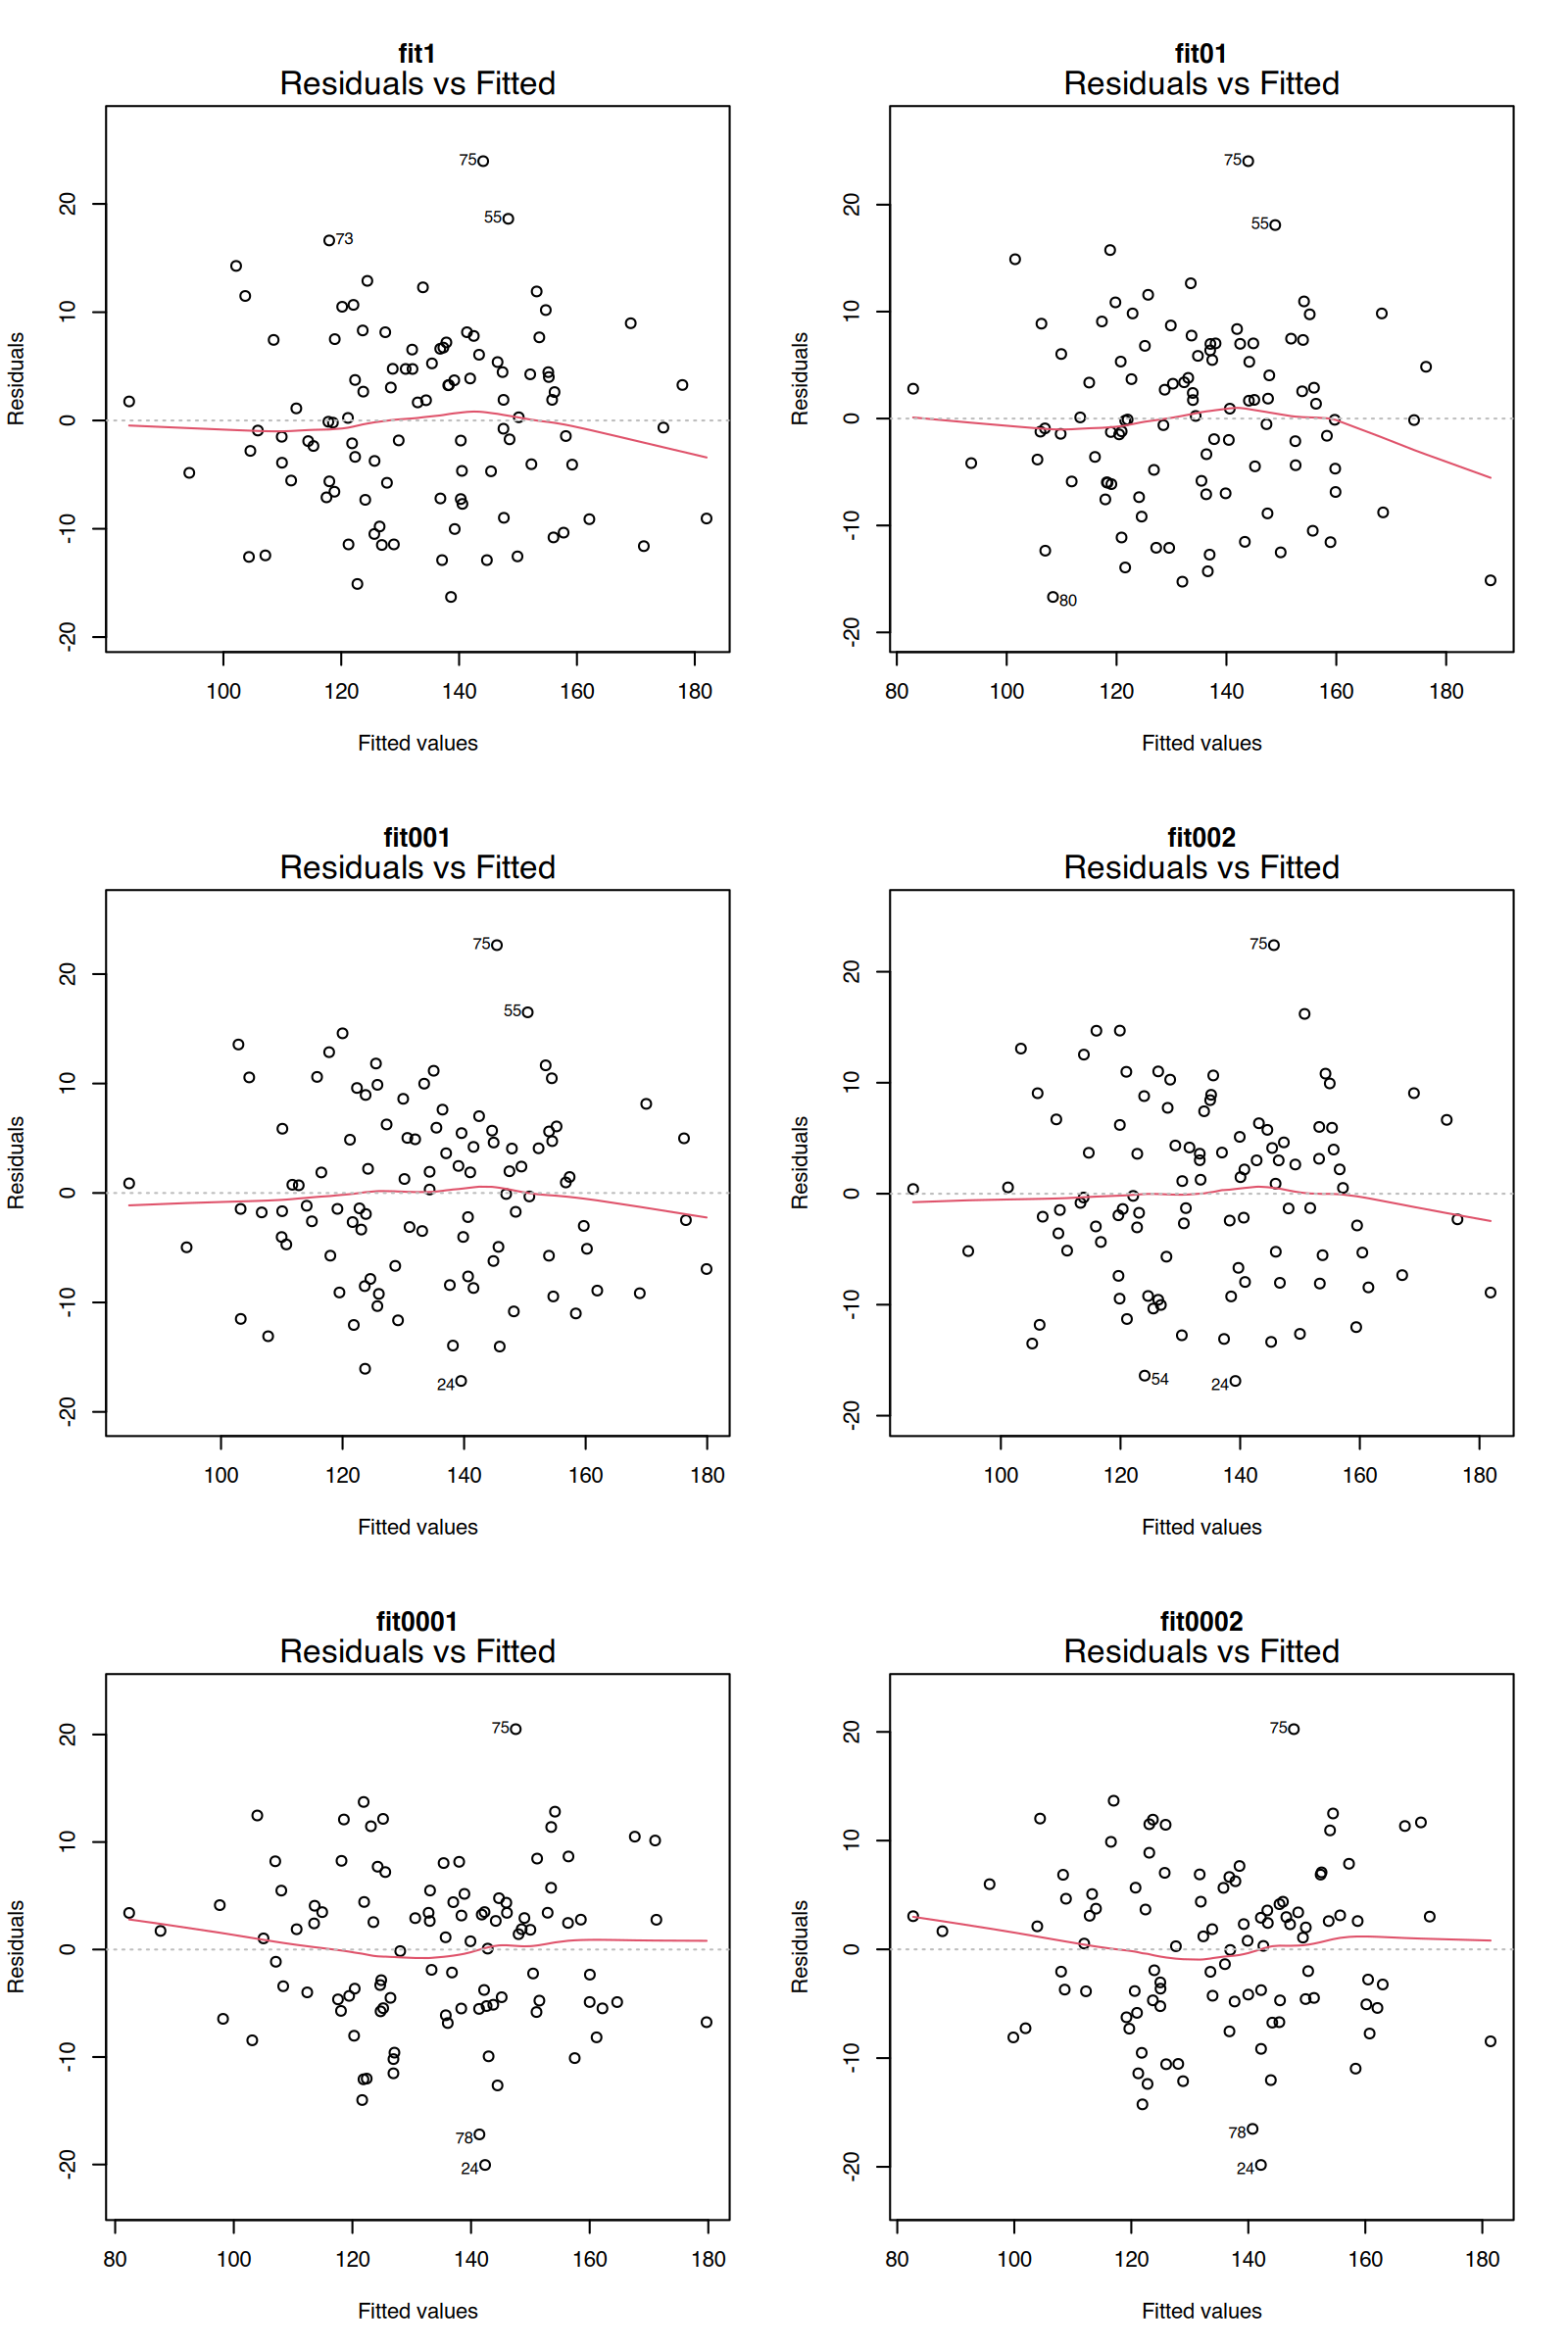
\includegraphics[width=0.88\linewidth]{figures/plottwists/diagnostics_1.png}
\caption{diagnostics 1}
\end{figure}

Nel nostro caso \texttt{\detokenize{fit002}} sembra il modello più aderente ai risultati desiderati per questo test. \texttt{\detokenize{fit0002}} ha un comportamento comunque accettabile, anche se mostra un maggiore rumore.

\subsubsection{2.3.2. Q-Q plot}
\label{sec:232-q-q-plot}

Il secondo grafico è il \textbf{Q-Q plot dei residui}, che confronta i quantili dei residui standardizzati con quelli teorici della distribuzione normale. Se l'ipotesi di normalità è ragionevole, i punti dovrebbero seguire approssimativamente la retta rossa tracciata con \texttt{\detokenize{qqline()}}. Come nei Q-Q plot della sezione 1.2, riportiamo anche il p-value del test di Shapiro-Wilk direttamente nel grafico.

\begin{figure}[H]
\centering
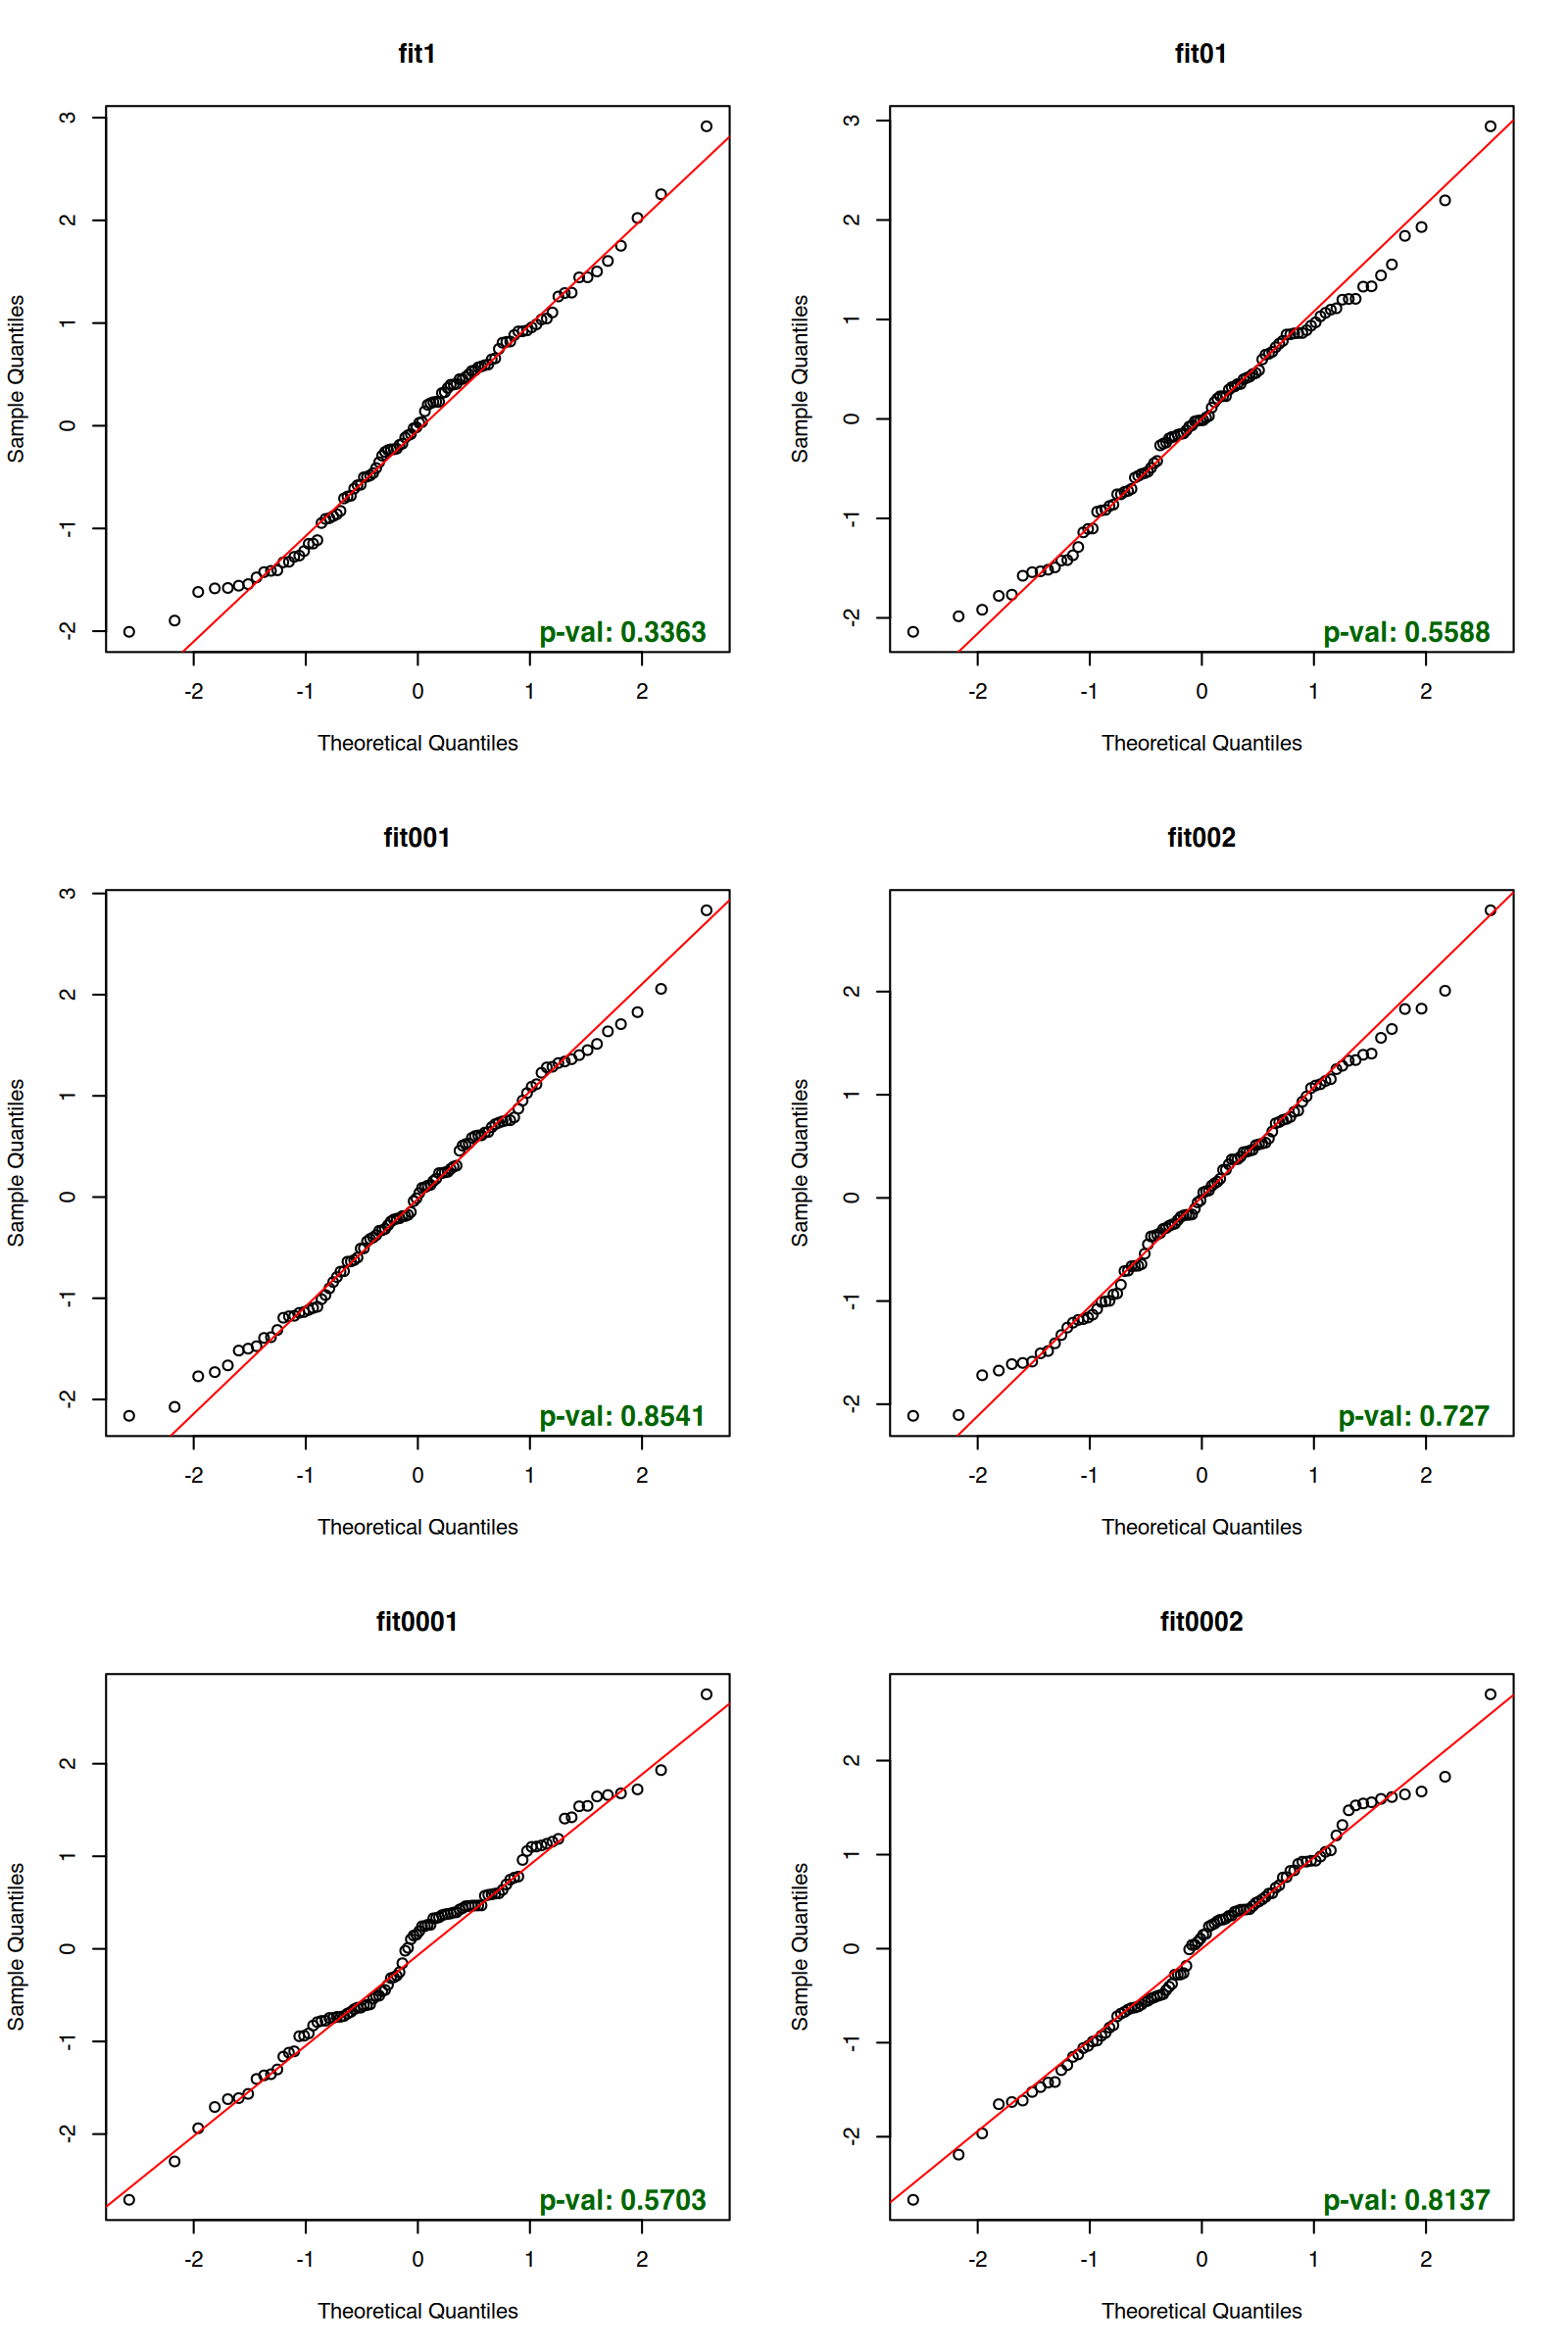
\includegraphics[width=0.88\linewidth]{figures/plottwists/diagnostics_2.png}
\caption{diagnostics 2}
\end{figure}

Qui \texttt{\detokenize{fit0002}} risulta tra i più convincenti: i punti seguono bene la retta, con scostamenti contenuti principalmente nelle code. Tuttavia, il test di Shapiro-Wilk sui suoi residui standardizzati mostra che, nonostante il risultato sia molto buono, \texttt{\detokenize{fit001}} ha una probabilità leggermente superiore di ottenere un campione con una distribuzione meno aderente a quella normale.

\begin{lstlisting}[style=rconsole]
# fit0002
W = 0.9919, p-value = 0.8137
# fit001
W = 0.99247, p-value = 0.8541
\end{lstlisting}

Dato che il p-value è molto maggiore di $\alpha = 0.05$, non rifiutiamo l'ipotesi nulla di normalità dei residui.

\subsubsection{2.3.3. Scale-Location}
\label{sec:233-scale-location}

Il terzo grafico è \textbf{Scale-Location}, che mette in relazione i valori stimati con la radice dei residui standardizzati in valore assoluto. Questo grafico serve a valutare l'omoschedasticità: in un modello ideale, la dispersione dei residui dovrebbe rimanere circa costante al variare dei valori stimati.

\begin{figure}[H]
\centering
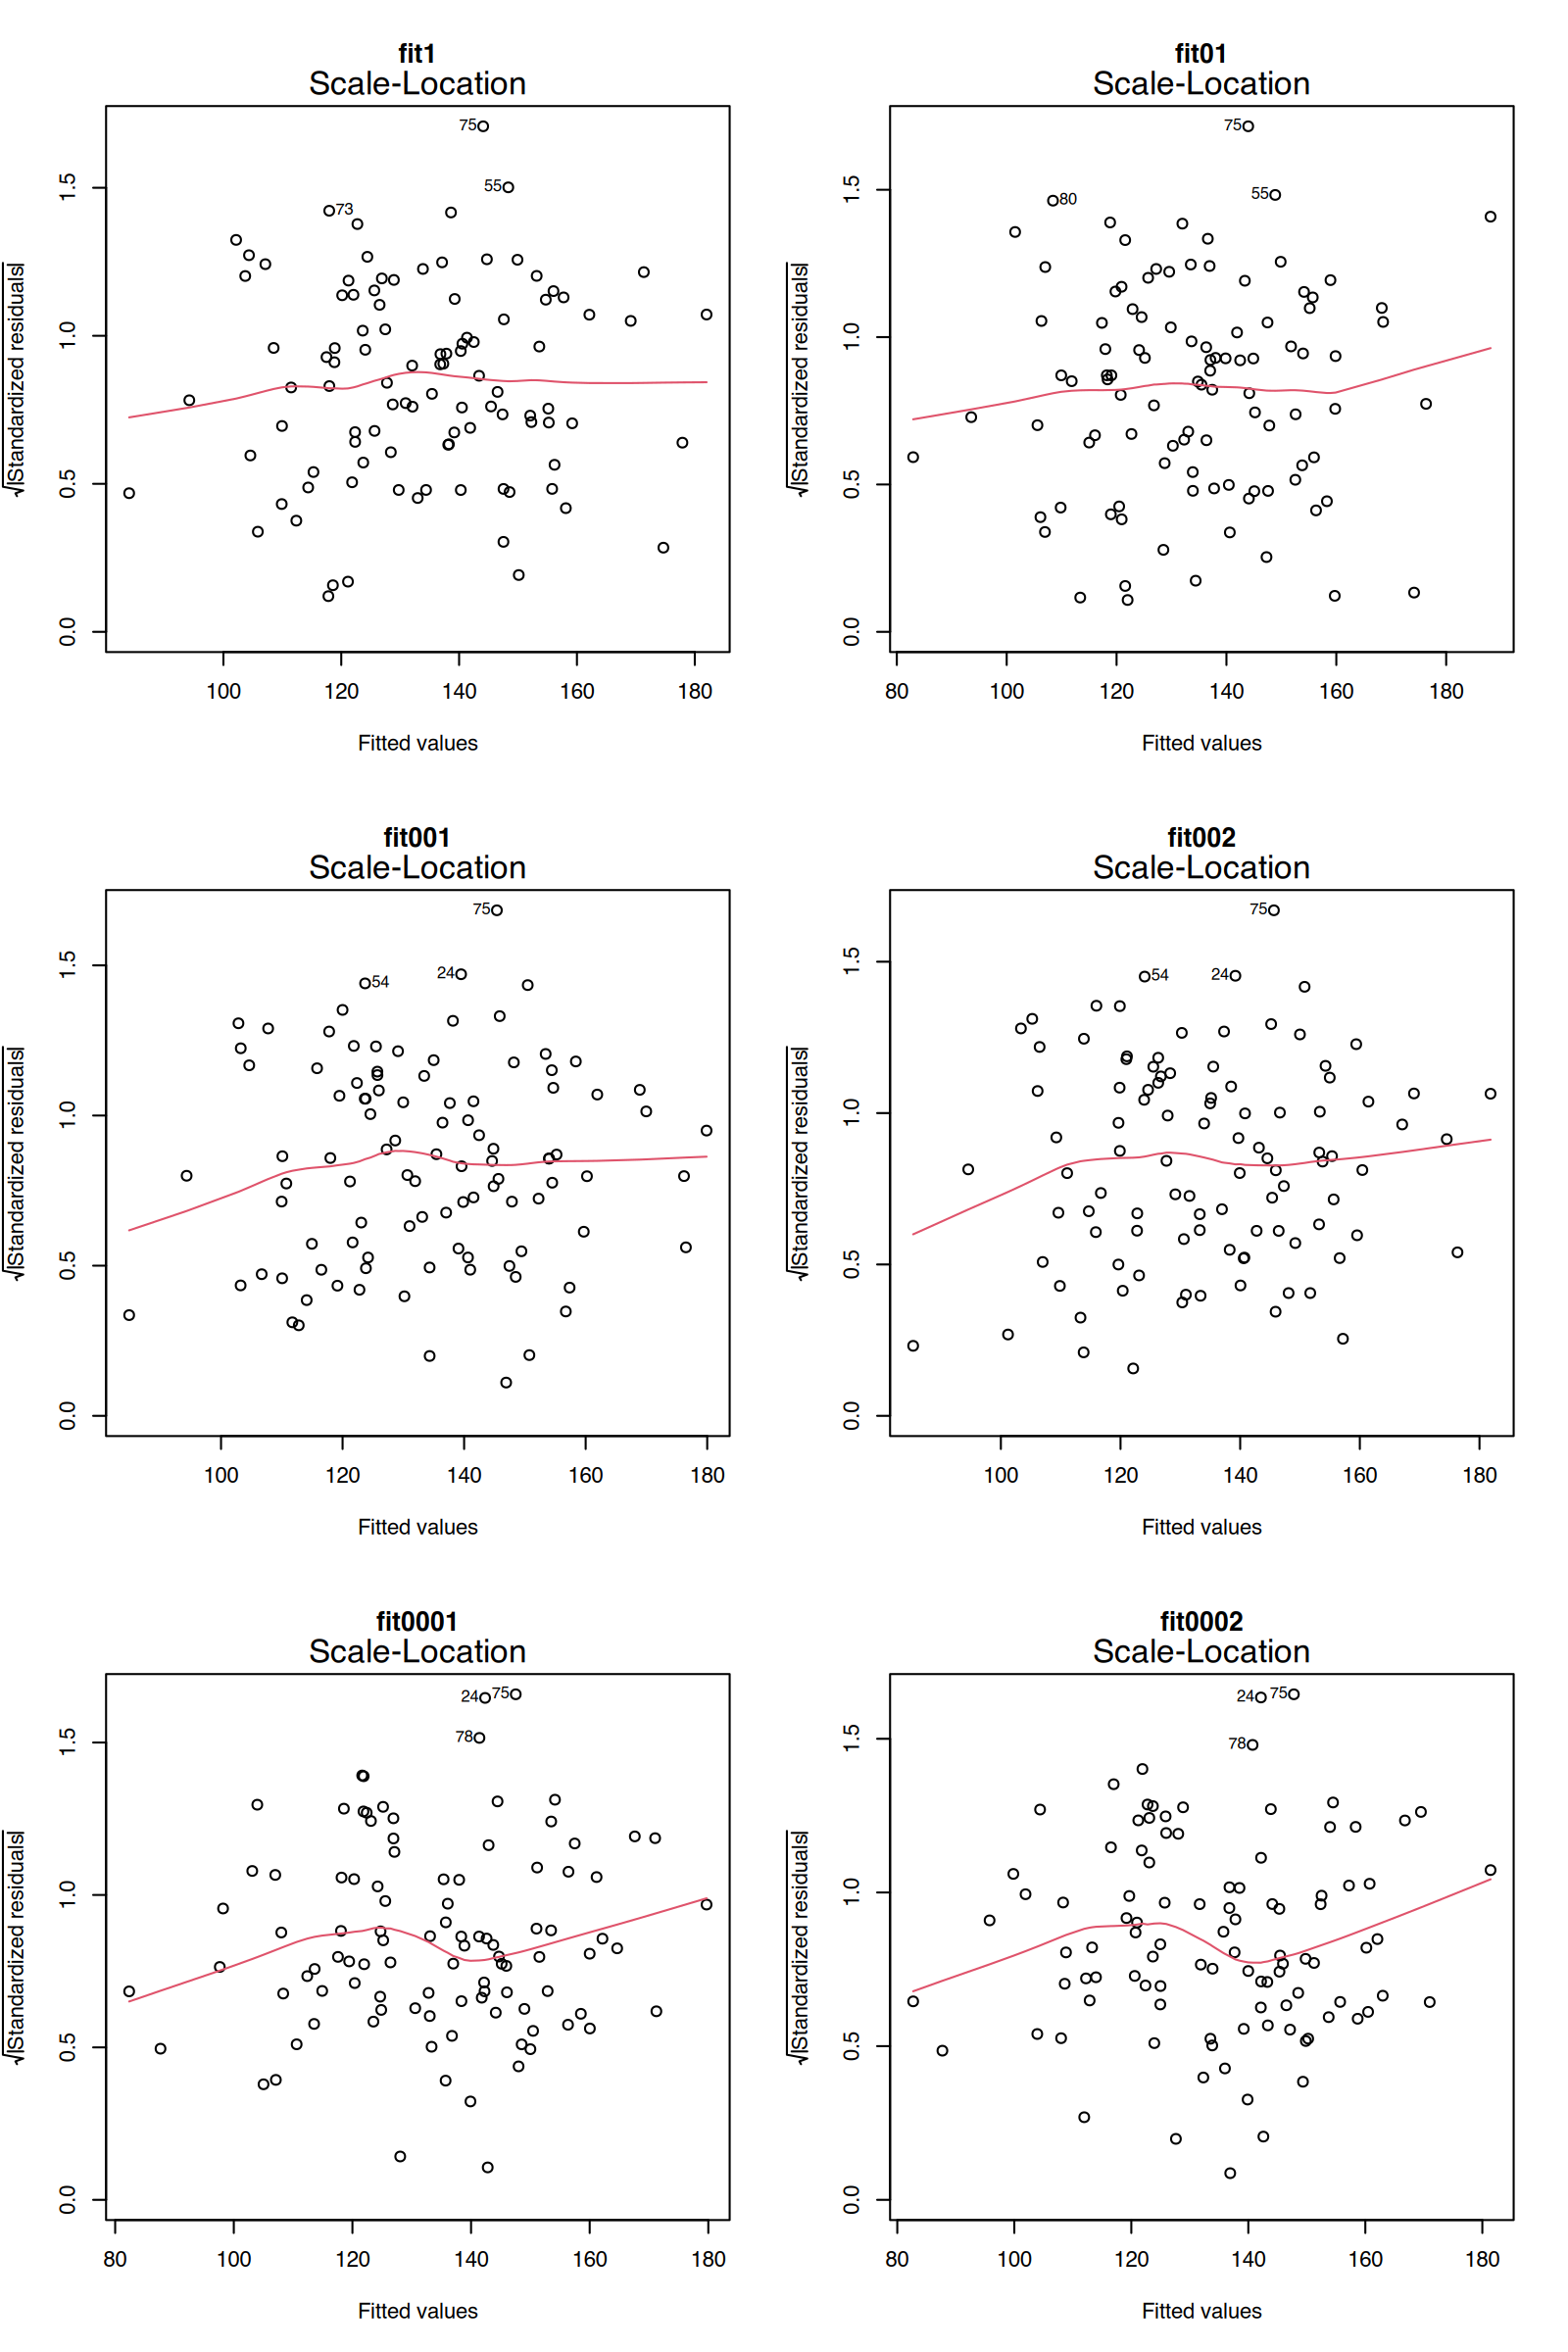
\includegraphics[width=0.88\linewidth]{figures/plottwists/diagnostics_3.png}
\caption{diagnostics 3}
\end{figure}

Da questo punto di vista \texttt{\detokenize{fit1}} e \texttt{\detokenize{fit01}} appaiono leggermente più regolari, perché la linea rossa è più stabile. \texttt{\detokenize{fit0002}} mostra invece una lieve crescita della dispersione per valori stimati più alti.

\subsubsection{2.3.4. Cook's Distance}
\label{sec:234-cooks-distance}

L'ultimo grafico è la \textbf{Cook's Distance}, che misura quanto ogni singola osservazione influenza la stima del modello. Una regola pratica è considerare con attenzione le osservazioni per cui:

\[
D_i > \frac{4}{n}
\]

Nel nostro caso, con $n = 100$, la soglia indicativa è $\frac{4}{n} = 0.04$.

\begin{figure}[H]
\centering
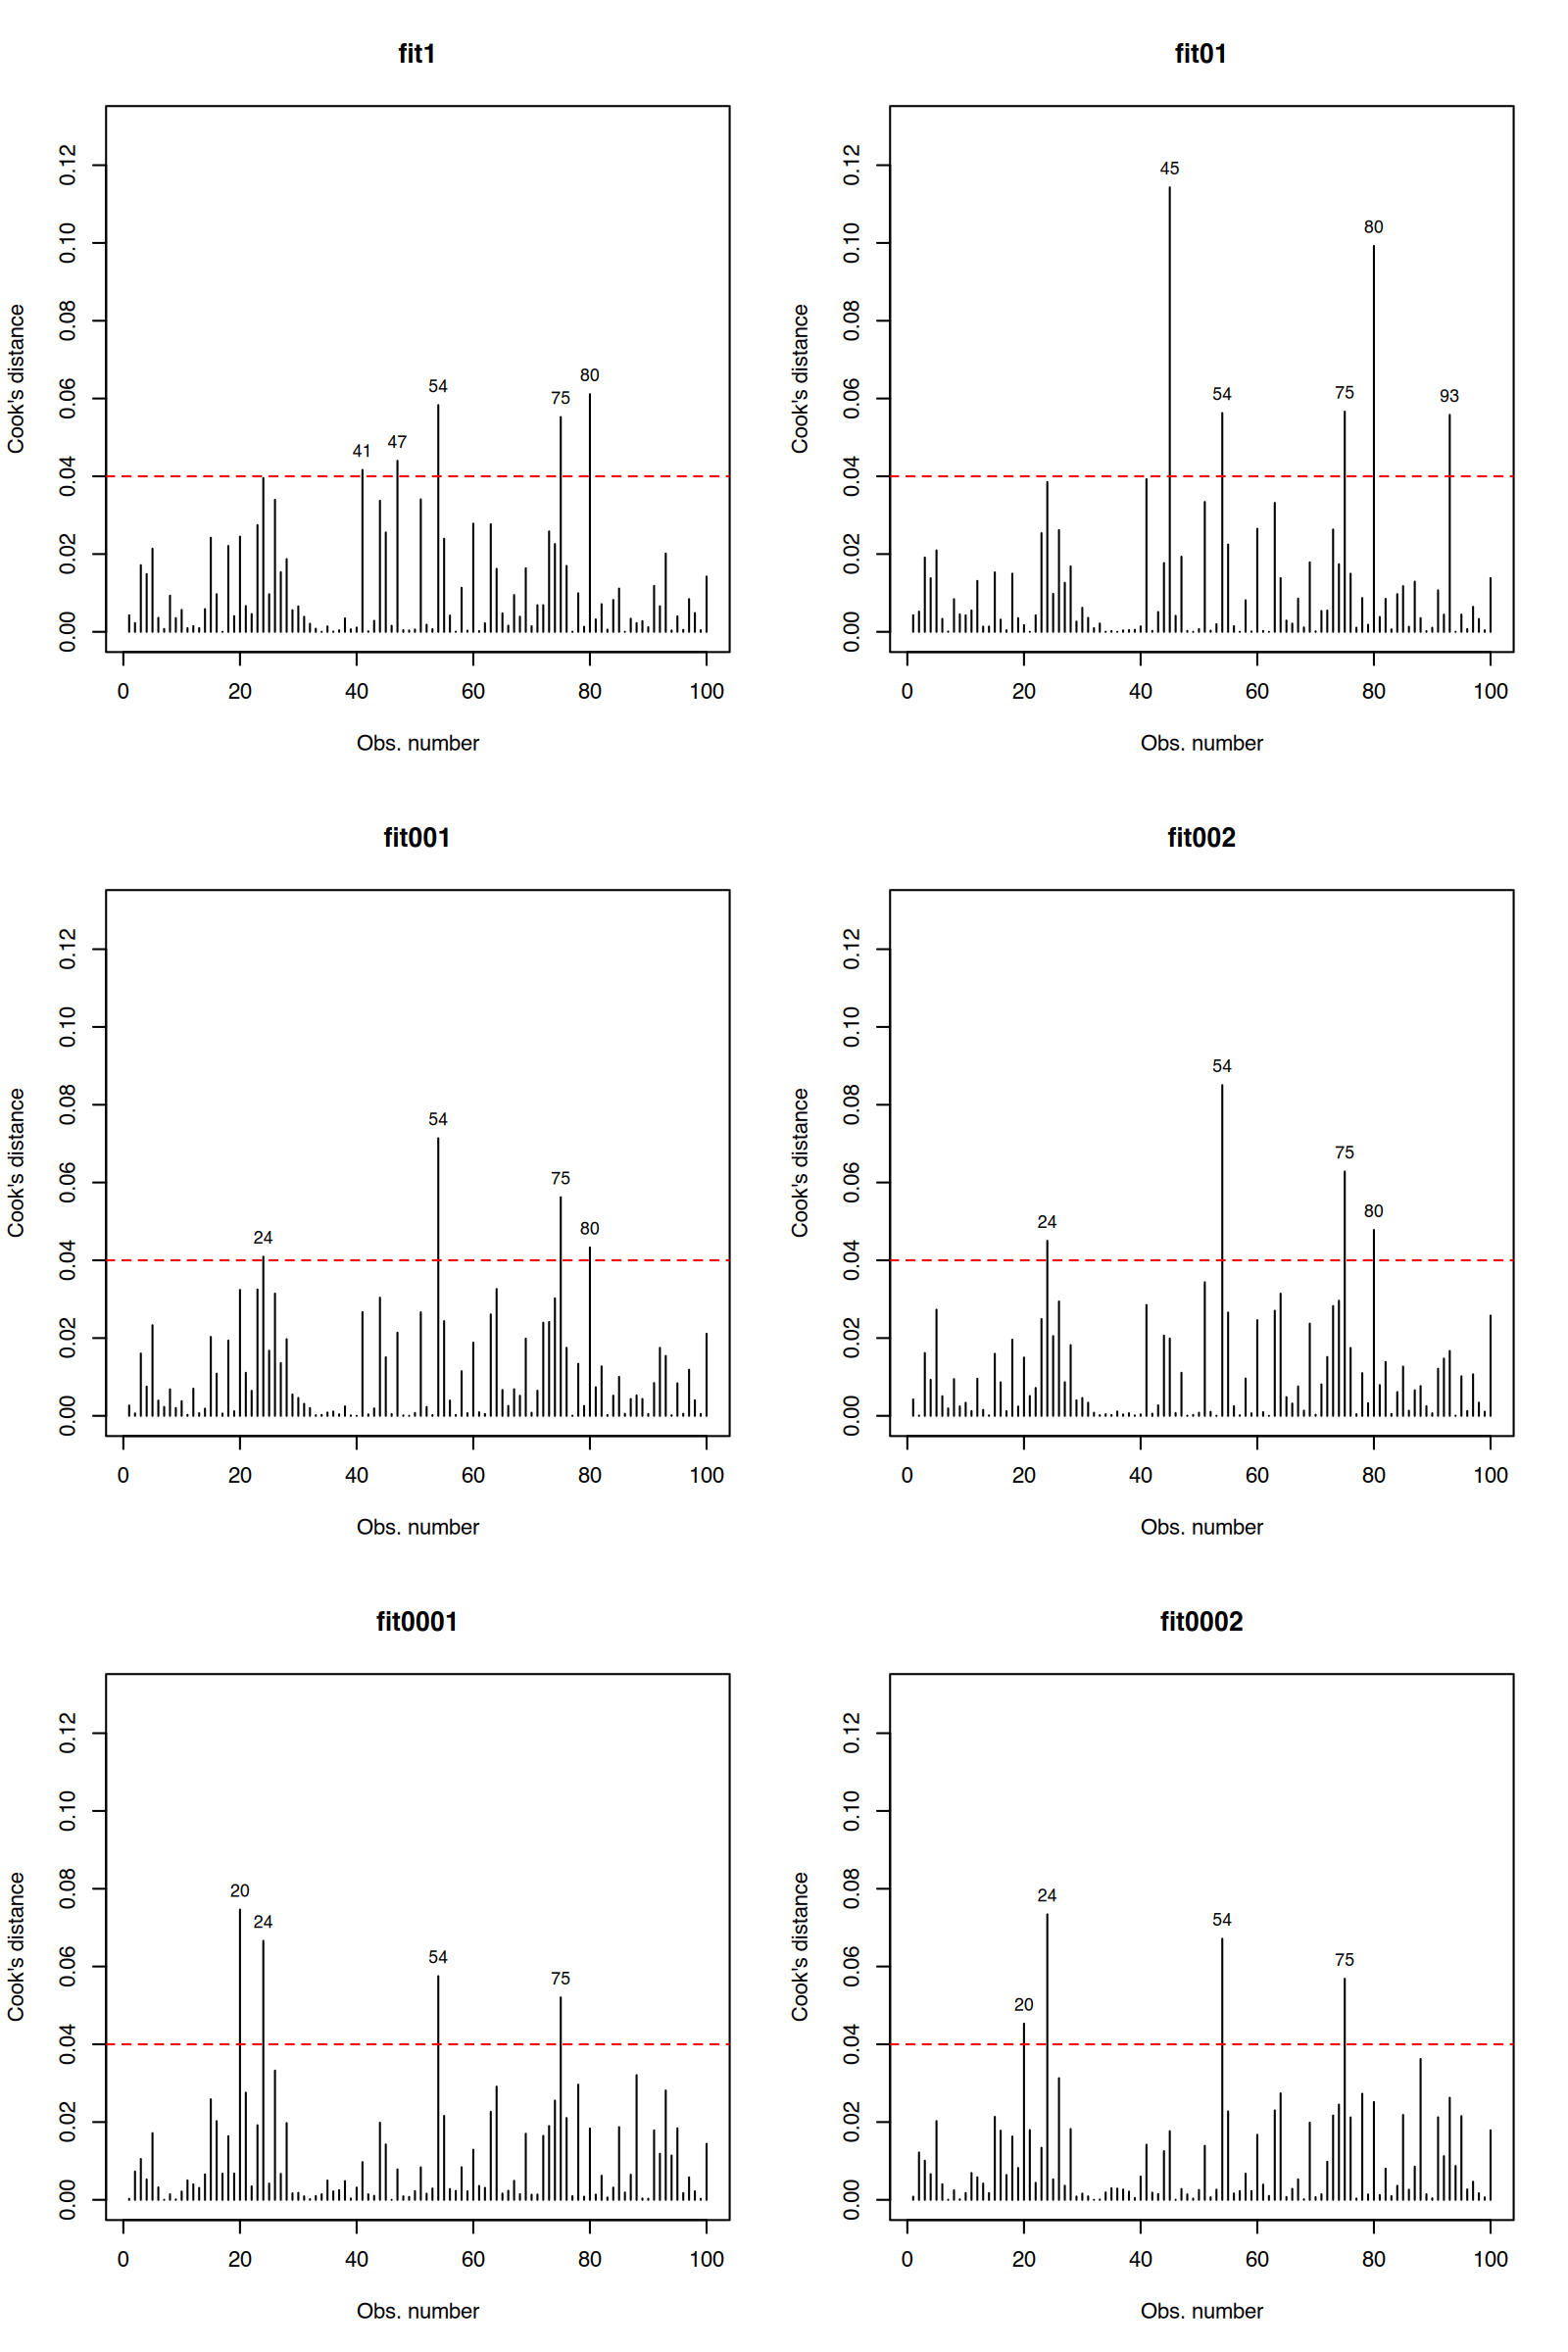
\includegraphics[width=0.88\linewidth]{figures/plottwists/diagnostics_4.png}
\caption{diagnostics 4}
\end{figure}

Per la distanza di Cook i modelli più interessanti sono \texttt{\detokenize{fit001}} e \texttt{\detokenize{fit1}}.

\subsubsection{2.3.5. Multicollinearità}
\label{sec:235-multicollinearita}

È possibile effettuare un'ulteriore analisi diagnostica su quanto i regressori siano correlati tra loro, ovvero la multicollinearità del modello (\texttt{\detokenize{vif(fitX)}}).

Per calcolare il VIF di ciascun regressore lo isoliamo come variabile dipendente, e ne prevediamo poi il valore tramite regressione lineare semplice, in funzione di tutti gli altri; questo valore indica quindi quanto quel singolo regressore sia spiegato dalle rimanenti variabili.

\[
1 \underset{\text{best}}< VIF_j = \frac{1}{1-R_j^2}
\]

\begin{lstlisting}[style=rconsole,caption={Multicollinearità di fit0002}]
    x1_ISO       x2_T      x3_MP     x6_GSI  I(x2_T^2) I(x7_UA^2)
  1.079947   1.079358   1.024063   1.051543   1.021741   1.066195
\end{lstlisting}

Come si può notare, il modello \texttt{\detokenize{fit0002}} non mostra segni di collinearità tra più variabili. Abbiamo trovato interessante mostrare un caso in cui i parametri del modello presentano un VIF non trascurabile. \texttt{\detokenize{vif(fit0000)}} restituisce ad esempio:

\begin{lstlisting}[style=rconsole,caption={Estratto dei VIF\textgreater{}5}]
        x5_F    I(x7_UA^2)
    7.439663      6.433935
\end{lstlisting}

Il valore del VIF di \texttt{\detokenize{x5_F}} si allinea con i risultati dell'\hyperref[sec:14-analisi-di-correlazione]{\sectionlink{analisi di correlazione}}, in cui vediamo chiaramente come \texttt{\detokenize{x5_F}} sia correlato con diverse altre variabili.

\subsection{2.4. Regressione Stepwise}
\label{sec:24-regressione-stepwise}

Un approccio alternativo alla costruzione del modello è quello di utilizzare una procedura automatica di selezione dei regressori, come la regressione stepwise. Questa tecnica permette di aggiungere o rimuovere regressori in maniera iterativa.

Nel nostro caso abbiamo usato uno scope massimo che contiene tutti i regressori lineari, tutte le interazioni a due variabili e i termini quadratici:

\[
y_{IQ} \sim (\text{x1\_ISO}+\text{x2\_T}+\text{x3\_MP}+\text{x4\_CF}+\text{x5\_F}+\text{x6\_GSI}+\text{x7\_UA})^2
+\sum_{j=1}^{7}x_j^2
\]

Abbiamo provato le tre direzioni disponibili in \texttt{\detokenize{step()}} usando sia il criterio AIC che BIC:

\begin{itemize}
\item \texttt{\detokenize{backward}}: parte dal modello completo e rimuove regressori;
\item \texttt{\detokenize{forward}}: parte dal modello nullo e aggiunge regressori;
\item \texttt{\detokenize{both}}: parte da un modello di mezzo, che contiene tutti i regressori lineari, e può sia aggiungere sia rimuovere regressori.
\end{itemize}

Il BIC corrisponde a una penalizzazione $k = \log{n}$, quindi penalizza la complessità più severamente dell'AIC, che usa invece $k = 2$, con numerosità campionaria $n \ge 8$.

\begin{lstlisting}[style=rconsole]
              SQE        R2       R2a     Fstat      AIC      BIC
backward_bic  5495    0.8666    0.8580    100.69    700.4    721.3
forward_bic   5495    0.8666    0.8580    100.69    700.4    721.3
both_bic      5495    0.8666    0.8580    100.69    700.4    721.3
backward_aic  4349    0.8944    0.8725     40.86    699.0    748.5
forward_aic   4912    0.8807    0.8688     73.85    695.2    723.9
both_aic      4912    0.8807    0.8688     73.85    695.2    723.9
\end{lstlisting}

Con il criterio BIC tutte e tre le direzioni portano allo stesso modello finale:

\[
\widehat{y}_{IQ}
= \beta_0 + \beta_1 \text{x1\_ISO} + \beta_2 \text{x2\_T} + \beta_3 \text{x3\_MP}
+ \beta_4 \text{x6\_GSI}
+ \beta_5 \text{x2\_T}^2 + \beta_6 \text{x7\_UA}^2
\]

Questo risultato è particolarmente interessante perché coincide con il modello scelto manualmente (\texttt{\detokenize{FLAG = fit0002}}). La procedura automatica conferma quindi che i regressori \texttt{\detokenize{x4_CF}}, \texttt{\detokenize{x5_F}} e \texttt{\detokenize{x7_UA}} lineare non portano un miglioramento sufficiente una volta considerati gli altri termini.

Con il criterio AIC, invece, i risultati dipendono maggiormente dal punto di partenza. Questo è coerente con il fatto che AIC penalizza meno la complessità rispetto a BIC: modelli più grandi possono essere mantenuti più facilmente, e la procedura stepwise può fermarsi in soluzioni diverse.

Partendo dal modello completo, \texttt{\detokenize{backward_aic}} conserva il modello più ampio:

\[
\begin{aligned}
\widehat{y}_{IQ}
=\;& \beta_0 + \beta_1 \text{x1\_ISO} + \beta_2 \text{x2\_T} + \beta_3 \text{x3\_MP}
+ \beta_4 \text{x4\_CF} + \beta_5 \text{x5\_F} + \beta_6 \text{x6\_GSI}
\\
&+ \beta_7 \text{x1\_ISO}^2 + \beta_8 \text{x2\_T}^2 + \beta_9 \text{x3\_MP}^2
+ \beta_{10} \text{x4\_CF}^2 + \beta_{11} \text{x6\_GSI}^2 + \beta_{12} \text{x7\_UA}^2
\\
&+ \beta_{13} \text{x1\_ISO}\cdot\text{x2\_T}
+ \beta_{14} \text{x1\_ISO}\cdot\text{x5\_F}
+ \beta_{15} \text{x2\_T}\cdot\text{x4\_CF}
\\
&+ \beta_{16} \text{x2\_T}\cdot\text{x5\_F}
+ \beta_{17} \text{x3\_MP}\cdot\text{x5\_F}
\end{aligned}
\]

Questo modello ha la SQE più bassa tra quelli ottenuti con la stepwise e il valore più alto di $R^2$, ma paga questa maggiore aderenza ai dati con una forte perdita di semplicità: il suo BIC arriva infatti a 748.5.

Partendo dal modello nullo (\texttt{\detokenize{forward_aic}}) e dal modello lineare intermedio (\texttt{\detokenize{both_aic}}), invece, AIC porta allo stesso modello finale:

\[
\begin{aligned}
\widehat{y}_{IQ}
=\;& \beta_0 + \beta_1 \text{x1\_ISO} + \beta_2 \text{x2\_T} + \beta_3 \text{x3\_MP}
+ \beta_4 \text{x4\_CF} + \beta_5 \text{x6\_GSI}
\\
&+ \beta_6 \text{x2\_T}^2 + \beta_7 \text{x6\_GSI}^2 + \beta_8 \text{x7\_UA}^2
+ \beta_9 \text{x3\_MP}\cdot\text{x4\_CF}
\end{aligned}
\]

Questo modello rappresenta una soluzione intermedia: è più complesso del modello BIC/manuale, perché reinserisce \texttt{\detokenize{x4_CF}}, aggiunge il termine quadratico di \texttt{\detokenize{x6_GSI}} e l'interazione \texttt{\detokenize{x3_MP:x4_CF}}; tuttavia è molto più compatto rispetto a \texttt{\detokenize{backward_aic}}. Inoltre, nella tabella ha l'AIC più basso tra i modelli stepwise riportati, pari a 695.2.

Nel complesso, la stepwise conferma che il modello BIC coincide con \texttt{\detokenize{fit0002}}, rendendolo la scelta finale più coerente con il criterio BIC. Il modello \texttt{\detokenize{both_aic}}/\texttt{\detokenize{forward_aic}} resta utile come confronto perché migliora l'adattamento ai dati, con un rischio maggiore di overfitting.

\subsection{2.5. Intervalli di Confidenza}
\label{sec:25-intervalli-di-confidenza}

Per completare il confronto tra i modelli, consideriamo gli intervalli di confidenza al 95\% dei coefficienti, calcolati tramite \texttt{\detokenize{confint()}}. L'intervallo di confidenza fornisce un insieme di valori plausibili per il parametro reale: se l'intervallo non contiene lo zero, il relativo coefficiente è coerente con quanto osservato nei test t del \texttt{\detokenize{summary()}}.

\subsubsection{2.5.1. Modello finale}
\label{sec:251-modello-finale}

\begin{lstlisting}[style=rconsole]
                 Estimate     2.5 %    97.5 %
(Intercept)      141.1581  138.0885  144.2276
x1_ISO            -9.8775  -11.4468   -8.3083
x2_T              -9.2344  -10.8914   -7.5773
x3_MP              5.9568    4.3639    7.5497
x6_GSI            -8.1953   -9.7878   -6.6029
I(x2_T^2)         -3.6453   -5.5382   -1.7525
I(x7_UA^2)        -4.0947   -5.8445   -2.3449
\end{lstlisting}

\begin{figure}[H]
\centering
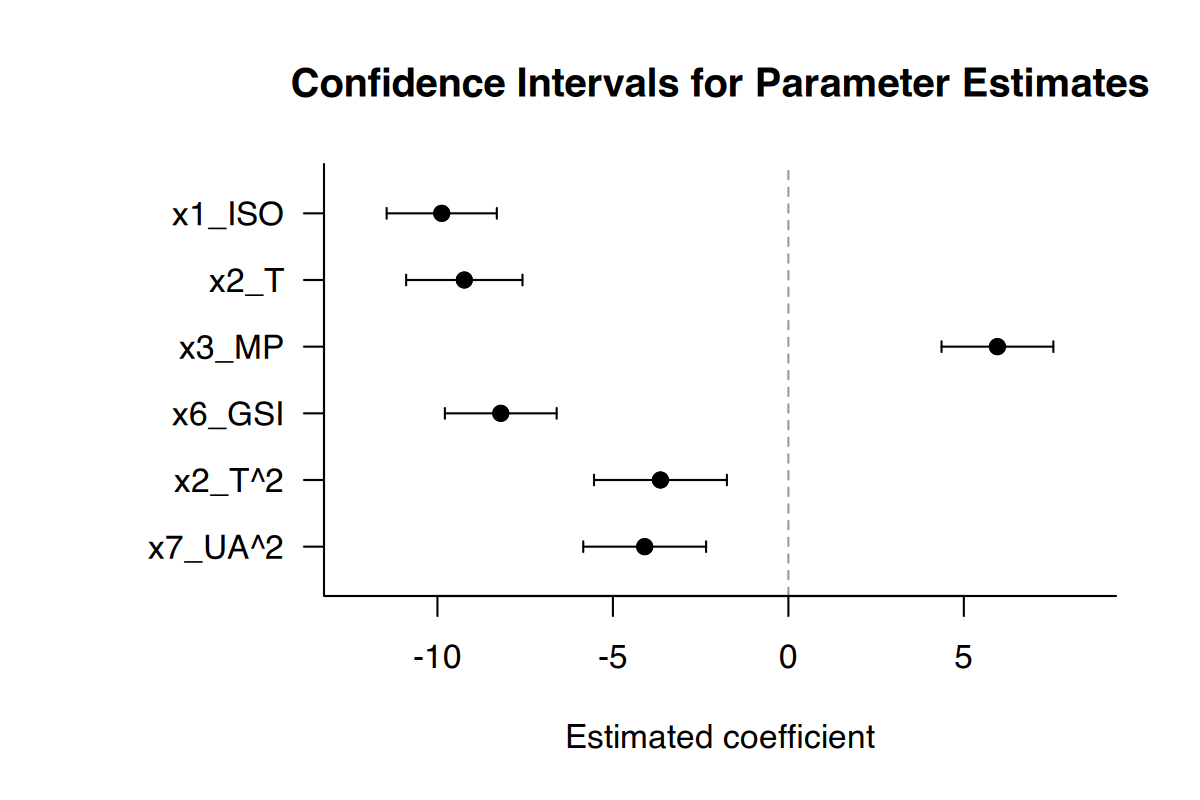
\includegraphics[width=0.60\linewidth]{figures/plottwists/confidence_intervals.png}
\caption{confidence intervals}
\end{figure}

Per il modello finale scelto (\texttt{\detokenize{FLAG = fit0002}}) osserviamo che tutti gli intervalli dei regressori mantenuti sono lontani da zero, il che rafforza la scelta di tale modello per rappresentare le relazioni tra le variabili.

\subsubsection{2.5.2. Modello stepwise backward AIC}
\label{sec:252-modello-stepwise-backward-aic}

\begin{figure}[H]
\centering
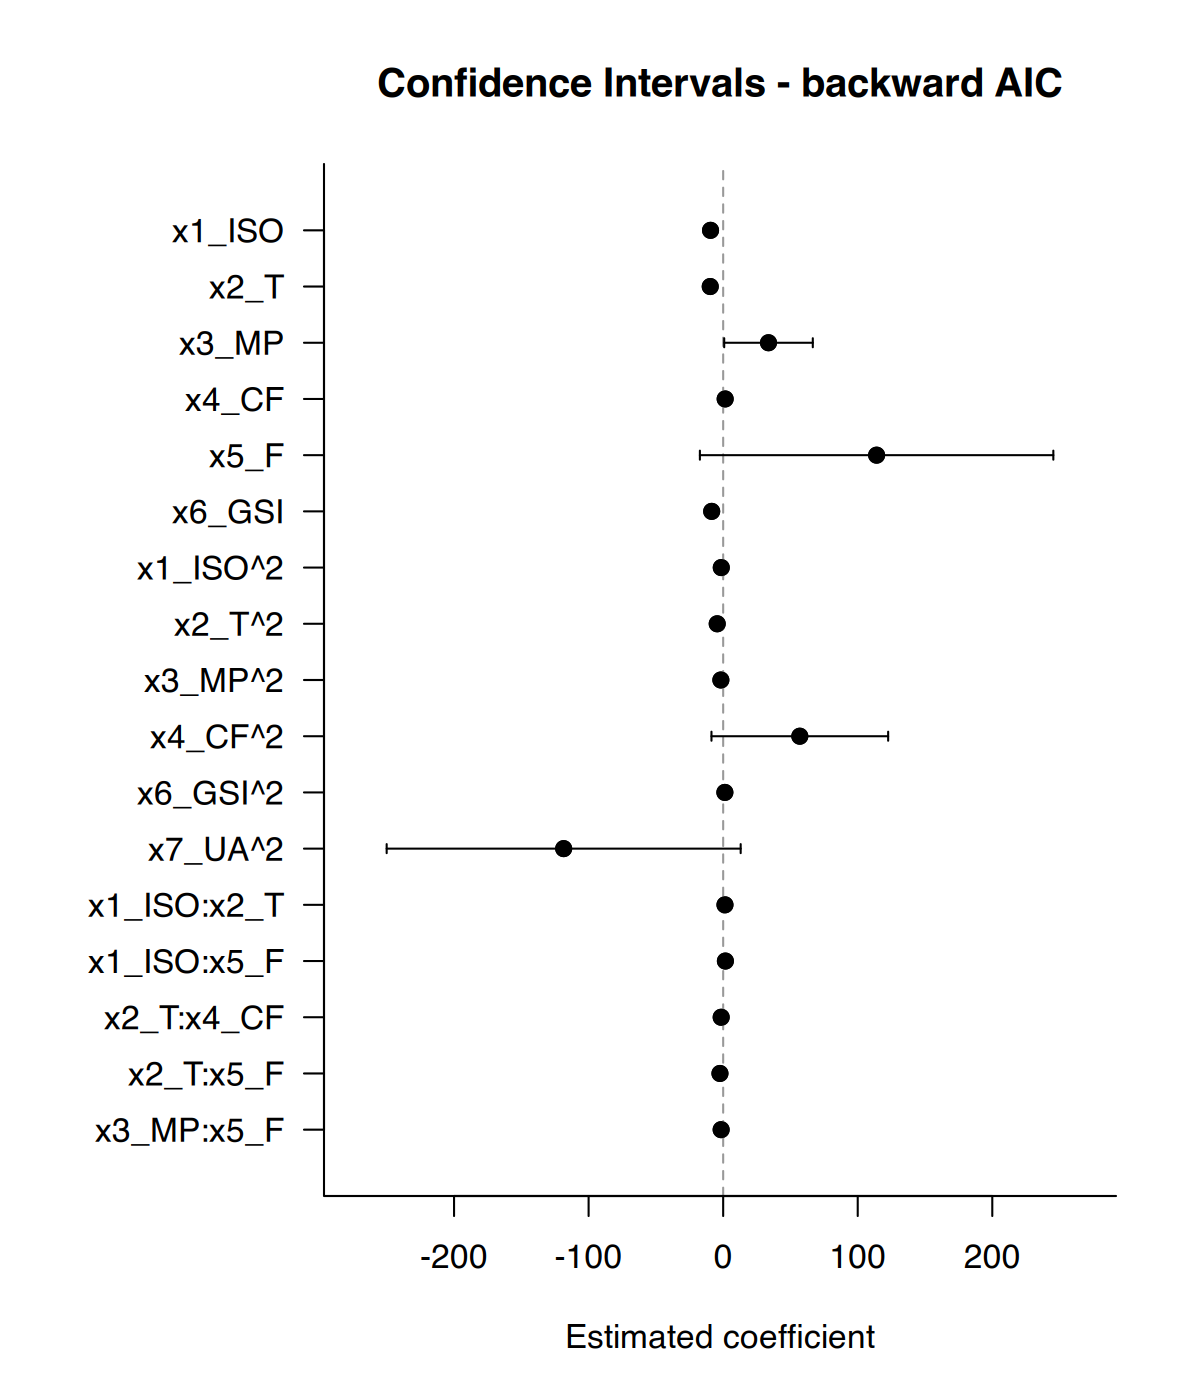
\includegraphics[width=0.60\linewidth]{figures/plottwists/confidence_intervals_backward_aic.png}
\caption{confidence intervals backward aic}
\end{figure}

Nel caso di \texttt{\detokenize{backward_aic}} si nota subito una maggiore instabilità. Alcuni coefficienti hanno intervalli molto ampi, e diversi intervalli attraversano lo zero (\texttt{\detokenize{x4_CF}}, \texttt{\detokenize{x5_F}}, tutti i quadrati inclusi tranne \texttt{\detokenize{x2_T^2}} e tutti i prodotti tranne \texttt{\detokenize{x2_T:x5_F}}). Questo significa che, pur avendo una SQE più bassa e un $R^2$ più alto, il modello contiene molti termini la cui stima è incerta.

\subsubsection{2.5.3. Modello stepwise both AIC}
\label{sec:253-modello-stepwise-both-aic}

\begin{figure}[H]
\centering
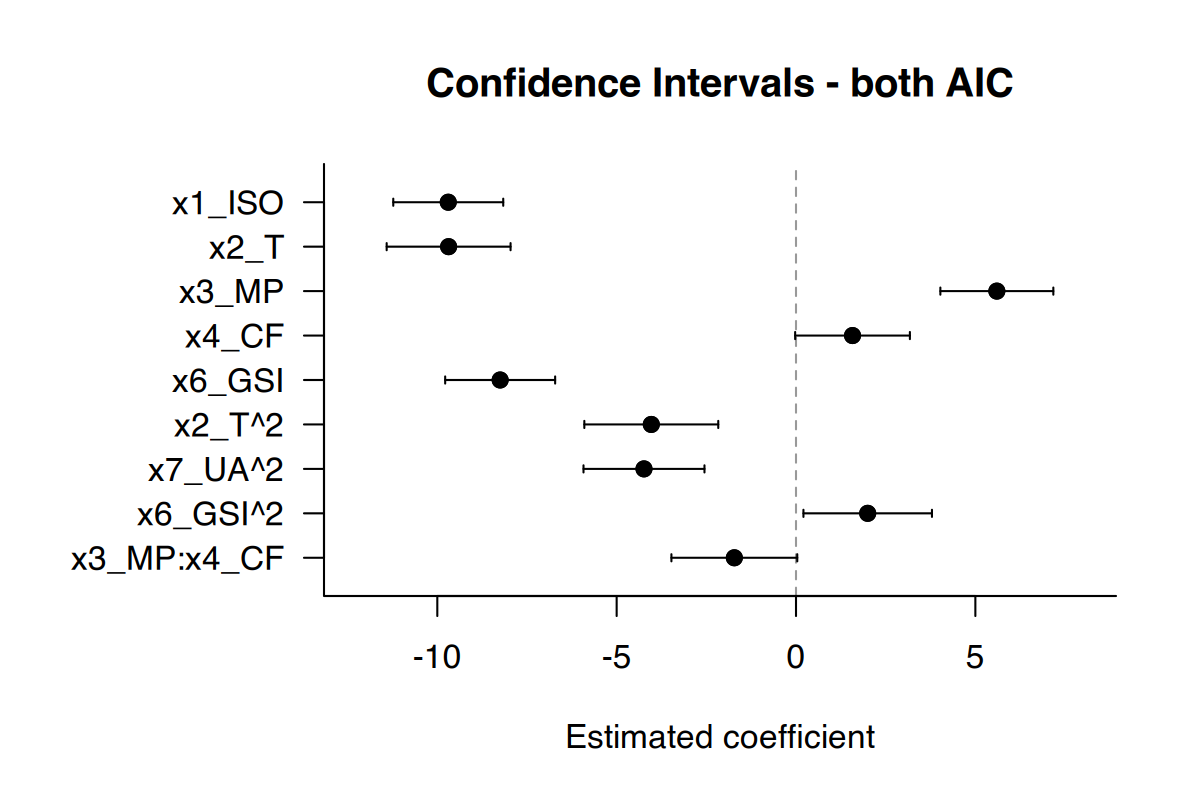
\includegraphics[width=0.60\linewidth]{figures/plottwists/confidence_intervals_both_aic.png}
\caption{confidence intervals both aic}
\end{figure}

Il modello \texttt{\detokenize{both_aic}} è notevolmente più leggibile e più compatto rispetto a \texttt{\detokenize{backward_aic}}, ma presenta comunque intersezioni con lo zero (\texttt{\detokenize{x4_CF}}, \texttt{\detokenize{x3_MP:x4_CF}}).

\subsection{2.6. Considerazioni finali}
\label{sec:26-considerazioni-finali}

In generale, gli intervalli di confidenza confermano quanto emerso dagli indici di confronto: i modelli AIC riescono ad adattarsi meglio ai dati osservati, tuttavia introducono termini meno stabili. Il modello \texttt{\detokenize{FLAG}}, invece, mantiene solo coefficienti con intervalli chiaramente separati da zero, risultando più semplice e più robusto dal punto di vista predittivo.

\section{3. Conclusioni}
\label{sec:3-conclusioni}

L'analisi descrittiva iniziale ha mostrato che le variabili indipendenti sono verosimilmente standardizzate, con media prossima a zero e deviazione standard prossima a uno, tuttavia solo \texttt{\detokenize{x5_F}} sembrerebbe essere normale per il test di Shapiro-Wilk. Dovremmo quindi tenere in considerazione per l'interpretazione finale che i coefficienti del modello non vanno letti come variazioni in unità fisiche originali, ma come effetti sulla scala trasformata del dataset.

Tra i modelli considerati, abbiamo scelto \texttt{\detokenize{FLAG}} come modello finale perché rappresenta il compromesso più convincente tra capacità esplicativa e semplicità. Il modello raggiunge un $R^2 = 0.8666$ e un $\text{BIC} = 721.3$, mantenendo solo sei termini:

\[
\begin{aligned}
Y =\;& 141.16 - 9.88 \cdot \text{x1\_ISO}
       - 9.23 \cdot \text{x2\_T}
       + 5.96 \cdot \text{x3\_MP}\\
     & - 8.20 \cdot \text{x6\_GSI}
       - 3.65 \cdot \text{x2\_T}^2
       - 4.09 \cdot \text{x7\_UA}^2 + \varepsilon
\end{aligned}
\]

Dal punto di vista operativo, se l'obiettivo è massimizzare la qualità dell'immagine \texttt{\detokenize{y_IQ}}, il modello suggerisce di lavorare verso valori bassi di \texttt{\detokenize{x1_ISO}} (sensibilità del sensore) e \texttt{\detokenize{x6_GSI}} (risoluzione al suolo in cm/px), e verso valori alti di \texttt{\detokenize{x3_MP}} (megapixel del sensore).

Per quanto riguarda \texttt{\detokenize{x2_T}} (tempo di esposizione), è presente sia come dipendenza lineare che quadratica. Mettendo le due in una sola funzione, risulta che è possibile massimizzare l'impatto positivo di \texttt{\detokenize{x2_T}} tramite valori (standardizzati) intorno a -1.26.

Per \texttt{\detokenize{x7_UA}} (altitudine di volo dell'UAV), invece, non rimane un effetto lineare ma solo un effetto quadratico negativo; di conseguenza il modello suggerisce di mantenerlo vicino a zero (standardizzato), evitando valori estremi in entrambe le direzioni.

Le variabili \texttt{\detokenize{x4_CF}}, \texttt{\detokenize{x5_F}} e il termine lineare di \texttt{\detokenize{x7_UA}} non compaiono nel modello finale. Questo significa che, una volta considerate le altre variabili, non apportano un miglioramento sufficiente da giustificare la loro presenza nel modello selezionato.

\emph{That's all folks.}
